\documentclass[french,a4paper,12pt]{report}
\usepackage[utf8]{inputenc}
\usepackage[T1]{fontenc}
%\Package paramétrage: marge horizontale à 2,5 cm, et la marge verticale à 1,5 cm.
\usepackage{geometry}
\geometry{hmargin=2cm,vmargin=3cm}
\usepackage{eso-pic}
\usepackage{graphicx}
\usepackage{float}
\usepackage{listings}
\usepackage{color}
\definecolor{dkgreen}{rgb}{0,0.6,0}
\definecolor{gray}{rgb}{0.5,0.5,0.5}
\definecolor{mauve}{rgb}{0.58,0,0.82}
\usepackage{pdfpages}
\usepackage{amsmath}

\lstset{frame=tb,
  language=Java,
  aboveskip=3mm,
  belowskip=3mm,
  showstringspaces=false,
  columns=flexible,
  basicstyle={\small\ttfamily},
  numbers=none,
  numberstyle=\tiny\color{gray},
  keywordstyle=\color{blue},
  commentstyle=\color{dkgreen},
  stringstyle=\color{mauve},
  breaklines=true,
  breakatwhitespace=true,
  tabsize=3
}

%\hfill\hbox to 0pt{\hss
\includegraphics[width=7cm]{UTBM_LOGO.png}\hss}\hfill\null\newline

\begin{document}

\title{	Université de Technologie de Belfort-Montbéliard \\
		{\large \textsc{Génie logiciel, spécialisé dans les systèmes embarqués }} \\
		\vspace{1cm}
		Laboratoire de Physique Nucléaire et des Hautes Énergies \\
		{\large \textsc{Contrôle Haptique et Asservissement de la Mécanique des Pianos de concert }}		
	  }
	  
\date{5 Février 2018 -- 13 Juillet 2018 }
	  
\author{Professeur suiveur : GECHTER Franck  \\
		Tuteur de stage		: LEBBOLO Hervé  \\
		Elève				: ROMET Pierre
		}

\makeatletter
  \begin{titlepage}
  \centering
  \
      {\large \textsc{ }}\\
      \textsc{}\\
      
      \vfill
       {\LARGE \textbf{\@title}} \\
    	\vspace{2em}     
      
    \vspace{1cm}
      {\large{	\@date\\
    \vspace{1cm}
       Stage ST50}}\\
    \vspace{1cm}
        {\large \@author} \\
    \vfill
        
\includegraphics[height=0.13\textheight]{UTBM_LOGO.png}
        \hfill
        
\includegraphics[height=0.09\textheight]{LPNHE_LOGO.png}
  \end{titlepage}
\makeatother

\tableofcontents
\parskip=5pt %to redefine line space of text only, and not for "tableofcontents"


%--------------------------------------------------------------------------------------
%
%	Avant Propos
%
%--------------------------------------------------------------------------------------
\part{Préambule}

  \chapter{Remerciement}
%  Tout d'abord je tiens à remercier l'ensemble de mes collègues pour l'accueille des plus chaleureux, au sein du laboratoire de physique nucléaire et des hautes énergies, ainsi que pour leur présence tout au long de mon stage, en m'aidant et me conseillant.
%  
%  Je voudrais remercier Monsieur Olivier LEDORTZ pour son aide concernant le langage VHDL.
%  
%  Je tiens à remercier mon maitre de stage Monsieur Hervé LEBBOLO, pour son implication dans l'encadrement de mon stage, son soutien, ainsi que pour l'ensemble des connaissances transmises dans le domaine de l'électronique analogique.
%  
%  Enfin, je tiens également à remercier mon enseignant suiveur, Monsieur Franck GECHTER, grâce à qui j'ai pu réaliser un stage de fin d'étude me permettant d'allier mon corps de métier, à une passion, la musique.
  
 \chapter{Introduction}

Dans le cadre des mes études d'ingénieur au sein de l'Université de Technologie de Belfort-Montbéliard, j'ai effectué un stage de fin d'études en laboratoire d'une durée de 24 semaines au sein du laboratoire de Physique Nucléaire et des Hautes Énergies à Paris.

Le laboratoire de Physique Nucléaire et des Hautes Énergies est une unité de recherche de l'institut national de  physique nucléaire et de physique des particules, institut du CNRS et des universités Sorbonne Université et Paris Diderot.

Mon stage s'est déroulé au sein du service électronique, sous la tutelle de Monsieur Hervé LEBBOLO.

Lors de ce stage, je fus recruté pour participer au projet "CHAMP"; projet interdisciplinaire, initié par Antoine LETESSIER SELVON, Hervé LEBBOLO, Philippe REPAIN, Laurent BESSIER, Thomas Hélie.

Ce projet interdisciplinaire associe de nombreuses compétences, en lutherie artisanale, en technique de préparation de piano, en physique, en électronique rapide et en mécanique de précision.

L'objectif est la réalisation d'un système de motorisation asservie de la mécanique d'un piano à queue afin d'offir de nouvelles couleurs aux préparateurs de pianos, ainsi que de nouvelles voies d'expression musicales aux interprètes tout en gardant intact le toucher traditionnel des mécaniques à répétition.

Le laboratoire étant spécialisé dans le domaine de l'électronique de précision et de l'électronique numérique, travaillant sur des projets tel que LSST (Large Synoptic Survey Telescope - Grand télescope d'étude synoptique), ce stage fut pour moi l'occasion d'évoluer dans un domaine des systèmes embarqués que je ne maitrisais peu, (de par ma formation) l'électronique analogique et numérique, ce qui m'a permis de découvrir et d'acquérir de nouvelles compétences ainsi que les méthodes de développement qui y sont liées.

Suite à cette introduction, nous allons poursuivre avec la présentation du laboratoire (LPNHE), puis nous conclurons cette première partie par la présentation du projet "CHAMP".


  
	\chapter{Présentation du laboratoire}
  Le LPNHE a été fondé par un groupe de chercheurs et enseignants-chercheurs issus de la division « hautes énergies » de l’institut de Physique Nucléaire (IPN) d’Orsay. En 1970, ces spécialistes des chambres à bulles rejoignent l’université Paris VI, puis l’ensemble devient un laboratoire associé au CNRS. À cette époque, la recherche s’y organise principalement autour d’expériences de chambres à bulles au CERN. Le LPNHE a donc derrière lui une longue histoire de collaboration avec le CERN.
  
  Aujourd’hui encore, même si les expériences et projets dans lesquels est engagé le laboratoire se trouvent maintenant sur les cinq continents, le CERN reste l’endroit privilégié où les chercheurs de physique des particules du laboratoire effectuent leur recherche.
  
  Le laboratoire de Physique Nucléaire et des Hautes Énergies est une unité de recherche de l'institut National de Physique Nucléaire et de Physique des particules, institut du CRNS et des universités Sorbonne Université et Paris Diderot. Il est constitué de 12 groupes de recherche, dont un à l’interface physique/biologie, de 3 services techniques (informatique, électronique, mécanique), et de deux services support étant l'administration et la logistique.
  
  Ces programmes couvrent les enjeux actuels de la physique des particules, des astroparticules, et de la cosmologie.
  On retrouve un groupe constitué de:
  \begin{itemize}
  \item  24 enseignant chercheurs
  \item  27 chercheurs
  \item  44 personnels d'appuis à la recherche
  \item  20 Doctorants
  \end{itemize}
  \newpage
  
  \section{Présentation des activités}
  Le laboratoire de physique nucléaire et des hautes énergies (LPNHE) est engagé dans plusieurs grands programmes expérimentaux, poursuivis dans le cadre de collaborations internationales auprès de très grandes infrastructures de recherche du monde entier, tel que des centres d’accélérateurs de particules, ainsi que des observatoires. Ces programmes couvrent les enjeux actuels de la physique des particules, des astroparticules, et de la cosmologie :
  
  On retrouve ainsi des travaux portant sûr:  
  \begin{itemize}
  \item L'origine des masses et des familles de particules, recherche du boson de Higgs, unification des interactions fondamentales, recherche de la supersymétrie, dimensions supplémentaires de l’espace-temps : thèmes abordés par les expériences CDF et D0 auprès du Tevatron à Fermilab, et par des expériences auprès du Large Hadron Collider au CERN (ATLAS au LPNHE), et enjeux d’un futur collisionneur e+e- pour lequel le LPNHE est engagé dans le développement de détecteurs en silicium.
  
  \item L’asymétrie matière-antimatière et la physique des saveurs lourdes : ce sont les sujets principaux des expériences BaBar au « SLAC National Laboratory », LHCb au CERN et la future SuperB factory en Italie.
  
  \item Les propriétés des neutrinos : participation à l’expérience Tokaï To Kamiokande (T2K) au Japon.
  
  \item Le contenu énergétique de l’univers, matière noire et énergie noire : le groupe Cosmologie du LPNHE joue un rôle déterminant dans Supernovae Legacy Survey (SNLS) auprès du Canadian French Hawaï Telescope dans Supernovae Factory (SNF) et est engagé dans la préparation des projets futurs Large Synoptic Survey Telescope (LSST) et EUCLID.
  
  \item L'origine des rayons cosmiques de très haute énergie : rayons gamma au TeV pour l’observatoire HESS en Namibie, et rayons cosmiques d’ultra haute énergie (10**18 eV) pour l’observatoire AUGER en Argentine.
  \end{itemize}
  
  Depuis la conception des expériences, en passant par l’étude et la réalisation des instruments de détection, la mise au point des systèmes de détection, d’acquisition et de réduction des données, la calibration et le monitorage des détecteurs pendant les longues périodes de prise de données, l’analyse et l’interprétation physique des mesures, pour enfin aboutir aux publications.
  Ce travail s'étale sur plusieurs années, parfois plus de dix ans, réunissant des équipes et développe des compétences extrêmement diversifiées en physique, électronique, informatique ou mécanique. 
  Les théoriciens du LPNHE représentent une petite composante qui enrichit la vie scientifique du laboratoire, ainsi que de la Fédération de Recherche sur les Interactions Fondamentales (FRIF), dont le laboratoire est membre, ce qui favorise un rapprochement plus fort théoriciens-expérimentateurs.
  
  \newpage
  
  \section{Projet et thématique}
  
		Entre 2015 et 2017, le laboratoire de Physique Nucléaire et des Hautes Energie (LPNHE) à travaillé, et continue de développer une vinghtaine de projet. Ces projets s'intègre dans différents domaines d'activité au sein du laboratoire que voici.
  	
  \begin{itemize}
		\item Masses et intéractions fondalentales
		
			- L'expérience Atlas, au LHC (Cern), est l'un des deux détecteurs polyvalents du grand collisionneur de hadrons (LHC). Il étudie des domaines de de physique très variés, de la recherche du boson de higgs, aux dimensions supplémentaires de l'espace-temps, en passant par les particules qui pourraient former la matière noire. Il regroupe un large ensemble de projet portant sur la désintégration du boson de Higgs, la physique du quark top, les sections efficaces de jets, de la calibration des électrons et des photons, du R\&D pour la fabrication d'un nouveau trajectographe ainsi que pour un "High Granularity Timing Detector".
			
			- Le projet CALICE, portant sur de la recherche et développement d'un nouveau calorimètre auprès de l'International Linear Collider (ILC). Le projet CALICE (Calorimeter for Linear Collider with Electrons) est un projet développé depuis quelques années pour concevoir des calorimètres de hautes granularité, ils pourront donc mesurer avec une grande précision le flux des particules et permettre de discerner les particules très proches lors du développement des gerbes, afin d'avoir un maximum d'informations sur toutes les désintégrations de particules.			
			
			- Le projet DZero, portant sur la physique du boson de Higgs et du top au Tevatron. Après la mise en évidence de la production de quarks top célibataire et la mesure de Delta Ms, la recherche du boson de Higgs est devenu l'enjeu majeur des expériences Dzero et CDF auprès du collisionneur TeVatron à Fermilab. 
			
		\item Asymétrie matière-antimatière
		
			- L'expérience LHCb (Large Hadron Collider Beauty) portant sur la physique des saveurs lourdes au LHC.
				LHCb explore les légères différences qui existent entre matière et antimatière grâce à l’étude d’un type de particule appelé « quark beauté » ou « quark b ». Au lieu d’utiliser un détecteur fermé au niveau du point de collision, tel que ceux d’ATLAS et de CMS, l’expérience LHCb a recours à plusieurs sous-détecteurs conçus pour observer principalement les particules émises « à petits angles », vers l’avant, dans le sens du faisceau.
			
			- L'expérience "BABAR", est une expérience de physique des particules réalisées au Stanford Linear Accelerator Center. Elle est dédiée à létudes de la physique des mésons B et de la violation de la symétrie CP dans leur désintégration faibles.
			
			- Le projet T2K, "T2K" pour Tokai to Kamioka est nouvel oscillateur à neutrons. Cette expérience de physique des particules situées au Japon, dans laquelle collabore de nombreux pays. Il s'agit d'une expérience d'oscillation de neutrinos, mesurant un faisceau de neutrinos muoniques à courte (280 m) et longue distance (295 km). Le but principal de T2K est de mesurer l'oscillation des neutrinos muoniques en neutrinos électroniques afin de mesurer le derniers paramètre de la matrice "Pontecorvo-Maki-Nakagawa-Sakata" permettant d'expliquer l'oscillation deneutrinos prédite par Bruno Pontecorvo en 1957.	
			
			- Le projet COMET, mettant en place des expérience de phénoménologie et la modélisation pour la physique des particules. L’expérience recherche la conversion cohérente sans neutrino d’un muon en électron dans un atome d’aluminium muonique, signal éventuel de physique au-delà du Modèle Standard.
			
			- Le projet SHiP (Search for Hidden Particles) est un projet d’expérience à cible fixe ayant comme projectiles les protons de 400GeV du faisceau du SPS (Super Proton Synchrotron) au CERN. Le détecteur est conçu avec une géométrie favorisant la recherche de particules dites invisibles. Ces dernières sont prédites par bon nombre de modèles théoriques et leur confirmation pourrait élucider certains des grands mystères de la physique actuelle tels que l’origine de la masse des neutrinos, de la matière noire ou encore de l’asymétrie baryonique de l’Univers. Ces modèles postulent l’existence de particules interagissant très faiblement avec celles du Modèle Standard comme par exemple les neutrinos stériles, les particules supersymétriques, les axions, ou encore les photons sombres.
			
		\item Rayonnement Cosmique et Matière Noire
			
			- Le projet AUGER.
			En 1938, P. Auger a mis en évidence l'existence de " grandes gerbes cosmiques atmosphériques contenant des corpuscules ultra pénétrantes, la technique utilisée etait celle des "compteurs en coïncidence ". Aujourd'hui l'observatoire Pierre Auger continue de founir à la communauté scientifique des données précises sur les gerbes atmosphérique les plus énergétiques jusqu'à E-10\^20 eV.
			
			- Le projet H.E.S.S est une expérience d'astronomie gamma dans le désert de Namibie. H.E.S.S est constituée de quatre télescopes atmosphériques à effet Cherenkov possédant chacun un miroir d’environ 12 mètres de diamètre, correspondant à un peu plus de 100 m2 de surface réfléchissante, placés aux quatre coins d’un carré de 120 mètres de côté. Ces télescopes opèrent entre environ 100 GeV et quelques dizaines de TeV. Au centre, un cinquième télescope équipé d’un miroir six fois plus grand en surface est sensible aux rayonnements de plus basse énergie, aux alentours de 20 GeV. 
			
			- L'expérience CTA (Cherenkov Telescope Array) constitue la prochaine génération de réseaux de télescopes à effet Cherenkov atmosphérique qui devrait prendre ses premières données à l’horizon 2022. Il a fait l’objet de la constitution d’une collaboration internationale de plus de 1300 scientifiques répartis dans 210i nstitutions de 32 pays. Ses objectifs sont de couvrir un domaine en énergie des rayonnements cosmiques détectés de dix GeV à plusieurs centaines de TeV avec une sensibilité accrue de plus d’un ordre de grandeur par rapports aux expériences existantes actuellement (essentiellement HESS, MAGIC et VERITAS).
			
			- L’expérience DAMIC (DArk Matter In CCDs) se propose de détecter le recul induit par la matière noire sur les noyaux de silicium composant les détecteurs à couplage capacitif (les CCD) qui servent habituellement de détecteur de photons en astronomie ou de particules en physique des hautes énergies. Le seuil de détection très bas des CCD (3.5 eV pour former une paire électron-trou) et la masse relativement faible du noyau de silicium permettent de sonder le domaine de masse des WIMP (Weakly Interacting Massive Particles) et d’autres candidats matière noire entre 1 et 20 GeV. Ce domaine en énergie est peu accessible aux grands détecteurs à liquide noble du fait de leur seuil de détection plus élevé.
						
			- Le projet DarkSide pour la recherche de matière noire repose sur l’utilisation d’une Chambre à Projection Temporelle (TPC) à l’Argon liquide en double phase. Un détecteur de 50 kg (DS-50) est actuellement en prise de données au LNGS. Il sera suivi par un détecteur de 20 t, DarkSide-20k.
			
			- Le projet XENON.
			Le détecteur XENON1T, développé par la collaboration XENON pour la recherche directe de matière noire, est l’expérience la plus sensible à l’heure actuelle dans la gamme de masse au-delà d’environ 10 GeV. Il est constitué par une TPC (Time Projection Chamber) remplie de 3.5 tonnes de xénon liquide, située dans le laboratoire souter-
rain du Gran Sasso, en Italie. Il vise à détecter la faible charge et la petite quantité de lumière qui devraient être émises à la suite de l’interaction d’une particule de matière noire avec un noyau de xénon. La construction de XENON1T a commencé en 2013 et s’est achevée en octobre 2015, suivie par une phase de mise en service et de calibration.
			
		\item Cosmologie et énergie noire
		
			- Le projet Supernovae, consiste en l'observation de supernova dans un gamme de redshift.
			
			- Le projet au sol "LSST", vise à l'observation répétée de l'ensemble du ciel visible, en s'affranchissant d'une partie des effets instrumentaux et atmosphériques. Il est basé sur un télescope au sol de 8.4 mètres de diamètre équipé d'une caméra de 3.2 milliard de pixels. L'ensemble, implanté au Chili, couvrira un champ de 9.6 degrés carrés sur le ciel balayé à la cadence d'un champ toutes les 40 secondes. Chaque champ sera ainsi visité 1000 fois durant les 10 ans de prise de données du programme.
			
			- eBOSS/DESI
			L’objectif principal du groupe est la mesure de l’échelle du pic acoustique des oscillations de baryons (BAO, pour Baryon Acoustic Oscillations), qui constitue un indicateur de distance angulaire et une mesure du taux d’expansion au redshift des sources analysées. On obtient ainsi une précision inégalée à haut redshift. Ce pic se mesure comme un excès de corrélation des traceurs de densités à une distance de séparation précise (en coordonnées co-mobiles).
			
			- Etude de la dynamique des systèmes auto-gravitants
			La motivation principale pour la recherche théorique du groupe est le problème de la formation des grandes structures de l’univers. Le défi large est de rendre compte systématiquement des observations pertinentes (distribution des galaxies, lentillage faible, CMB etc.) dans le cadre de la cosmologie standard (« Lambda CDM ») ou de ses variantes, et notamment dans le régime « non-linéaire ». L’accent de la recherche du groupe porte sur des questions fondamentales théoriques dans ce contexte, et il s’attache notamment à comprendre la dynamique non-linéaire de la matière purement gravitante et non-relativiste, approximation valable pour une grande partie de l’évolution de l’univers dans le modèle standard.		
		  	
  \end{itemize}
  
    
%--------------------------------------------------------------------------------------
%
%	Présentation du projet "CHAMP"
%
%--------------------------------------------------------------------------------------
\part{Qu'est ce que le projet "CHAMP" ?}
  \chapter{Présentation}
  
  Ce projet est né de la rencontre de Laurent BESSIÈRES, préparateur de piano intervenant pour les concerts et récitals de la Philarmonoe de Paris, et de Antoine LETESSIER SELVON, physicien des hautes énergies, directeur de recherche au CNRS et pianiste amateur. 
  
  De leur discution est né un projet au travers du quel ils cherche à élargir les possibilités de l'instrument en modifiant de mainère original sa mécanique. C'est en s'appuyant sur des techniques modernes qu'il souhaite proposer de nouveaux moyen d'expression aux artistes, tout en respectant le lien étroit qu'ils entretiennent avec leur instrument nottament au travers du toucher.
  
  \section{État de l'art}
  
  C’est en 1700 que Bartolomeo Cristofori invente la mécanique à échappement et construit le premier instrument à cordes frappées : le piano-forte. Ce sont les balbutiements de l’histoire du piano à queue. Le piano-forte révolutionne la technique pianistique car il permet à l’interprète de passer par le jeu des doigts, d’une nuance piano à une nuance forte, ouvrant de nouvelles voies à l’expression musicale et à la créativité des compositeurs. Cent vingt-trois ans plus tard, en 1821, Sébastien Érard ajouta un système de répétition à la mécanique de Cristofori et invente la mécanique moderne dite (improprement) à double échappement.

A la même époque, deux progrès techniques et industriels vont donner naissance au piano moderne. D’une part l’utilisation d’acier fondu pour les cordes et d’autre part l’introduction de cadres métalliques en fonte. Par ailleurs, de nombreux brevets seront déposés concernant la table d’harmonie, le croisement des cordes, le chevalet, l’assemblage de la mécanique, etc. 

De telle sorte, que peu avant 1890, l’essentiel de ce qui fait un piano moderne est accompli. A partir de cette date et à la suite d’une concentration industrielle de plus en plus forte, la nécessité de produire le plus d’instruments possible au moindre coût pour garantir plus de parts de marchés, les innovations vont essentiellement cesser et conduire en moins d’un siècle à la disparition de presque tous les facteurs artisanaux et à l’uniformisation quasi totale des instruments avec pour référence le piano de concert Steinway dont le modèle produit en 1877 réunissait déjà les inventions les plus importantes du XIXe siècle.

\newpage
On peut légitimement se demander quelles sont les lacunes du Steinway d’aujourd’hui, joué par 95\% des pianistes de la planète, qui justifieraient de bouleverser l’état actuel.
De fait, nous ne souhaitons pas nous appuyer sur d’éventuelles lacunes du Steinway ou d’ailleurs de tout autre piano, nous voulons avant tout ouvrir de nouvelles pistes. 
 Ceci en introduisant une source extérieure d’énergie, totalement et délicatement pilotée par l’instrumentiste, nous allons libérer des contraintes auquelles les pianos modernes, les Steinway en particulier, ont répondu de manière optimale, mais qu’ils ont malgré tout intégré.
 
 \section{Motivations}
 
 La mécanique à répétition de Sébastien Érard, brevetée à Londres par son neveu Pierre en 1921, est toujours utilisée aujourd’hui. Pourtant, la demande contemporaine de piano de concerts d’une puissance toujours plus grande (sans perte de sensibilité) n’a jamais été aussi forte. Par ailleurs, au cours des 30 dernières années, des facteurs indépendants ont introduit des innovations (nouveaux alliages pour les cordes, nouvelle structure pour le cadre et la table d’harmonie, etc) et repensé certains des choix techniques de la fin du XIXe siècle (croisement des cordes, barrage,...). Ainsi en France, Stephen Paulello, le dernier facteur français de pianos de concert en activité, vient de produire le premier exemplaire de sa dernière création : l’Opus 102. Ce piano de concert fait 3m de long et possède une tessiture de 102 notes (contre environ 2m80 et 88 notes pour les pianos de concert standard). Il comporte de nombreuses innovations et a été accueilli par la critique comme la “Bugatti Royale” des pianos.

La mécanique, de son coté, a peu évolué. L’utilisation de matériaux composites ou la modification de certaines pièces a parfois permis d’explorer quelques pistes (légèreté, coût, endurance, reproductivité) mais de manière limitée car le compromis actuel semble optimal compte tenu des contraintes imposées par la morphologie de l’instrument et de l’énergie qu’un artiste peut raisonnablement fournir pour l’actionner. Compte tenu de ces contraintes, l’ouverture vers de nouvelles expressions sonores par le biais de la mécanique ne semble pas
avoir été explorée. Certains développements ont consisté à introduire des éléments passifs, aimants, ressorts, élastiques, à l’intérieur de la mécanique ou sous les touches, mais aucun n’a semblé apporter suffisamment pour emporter l’adhésion des techniciens et surtout des artistes.\newline

	\begin{figure}[!ht]
    \center
    %\hfill\hbox to 0pt{\hss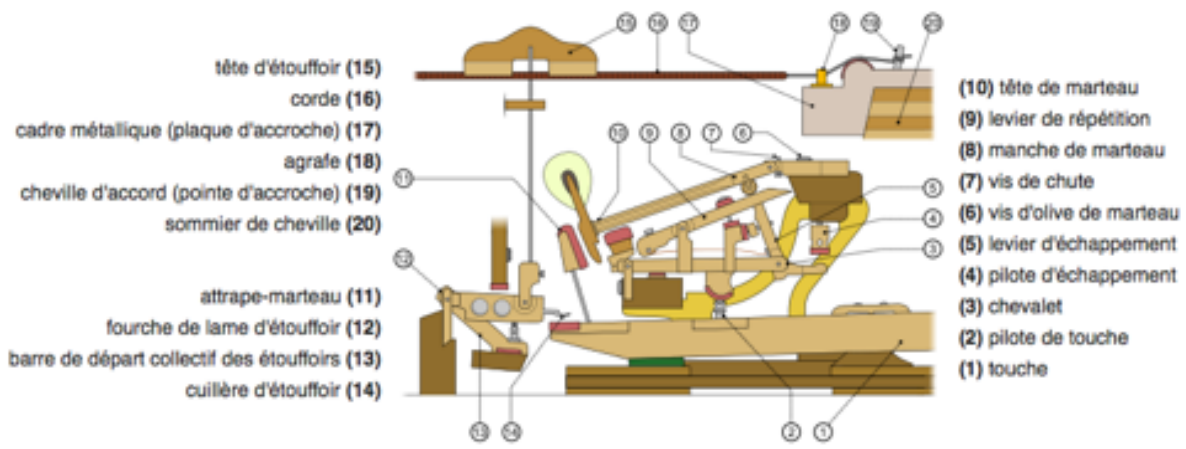
\includegraphics[width=15cm]{MECA_PIANO.png}\hss}\hfill\null
    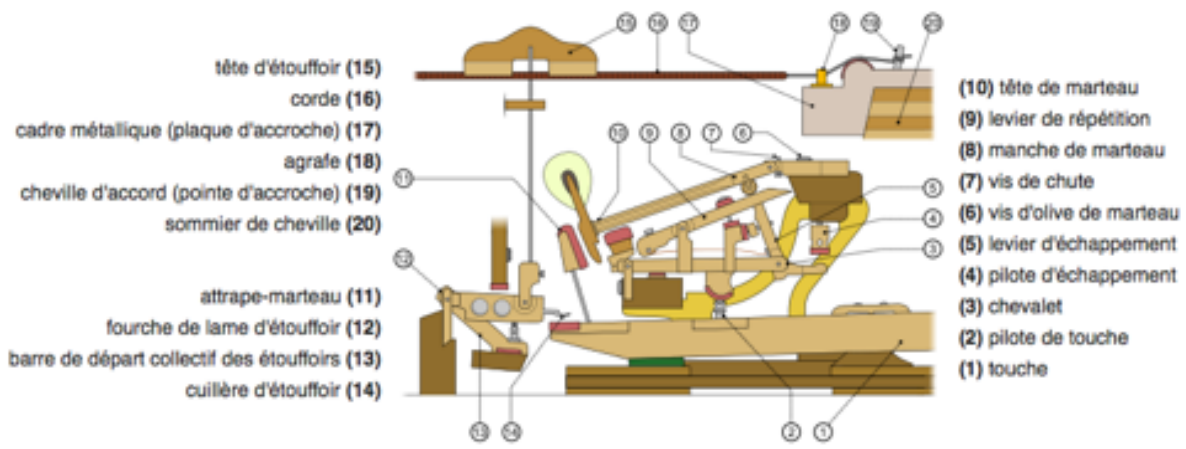
\includegraphics[width=15cm]{MECA_PIANO.png}
    \caption{Schéma de mécanique de Piano}
	\end{figure} 

Côté éléments actifs, l’essentiel des innovations concerne la reproduction autonome par l’instrument d’une musique jouée précédemment (sur lui même ou sur un instrument similaire), c’est la cas par exemple de la technologie "DisklavierTM" mise au point par Yamaha. Il n’y a pas d’interaction directe entre l’artiste et la mécanique augmentée. La mécanique de ces pianos enregistre le jeu de l’artiste puis le restitue sans son aide, avec une
perte de sensibilité notable. Il n’y a donc pas d’exploration de nouvelles capacités sonores ou d’augmentation de la palette de couleur de l’instrument, bien au contraire. Notons cependant les explorations de certains chercheurs comme par exemple Andrew McPherson6 et son “Magnetic Resonator Piano” où des électroaimants placés au dessus des cordes les maintiennent en résonance sous le contrôle de l’interprète offrant ici très clairement de nouvelles options d’expression.

D’un autre côté, les salles de concerts sont de plus en plus grandes et demandent, malgré une acoustique souvent exceptionnelle, des instruments de plus en plus puissants. Notons également que les orchestres sont aussi plus larges et que les instruments eux-mêmes, des cordes aux cuivres, ont également gagné en puissance. Ainsi on trouve aujourd’hui des pianos de plus de 3m (Fazioli 3,08m) permettant en principe d’obtenir une puissance extrême mais
c’est toujours la mécanique de Sébastien Érard qui est employée pour produire le son, une mécanique à la puissance limitée par celle que l’artiste peut lui fournir.

La puissance n’est cependant que l’un des paramètres sur lequel l’addition d’une source extérieure d’énergie permet d’intervenir. À puissance fixe, on peut explorer une répartition différente de l’énergie cinétique entre la masse du marteau et sa vitesse. Cette exploration est très limitée dans le cas d’une mécanique traditionnelle car l’inertie de l’ensemble doit être contenue afin que l’effort d’enfoncement des touches reste tolérable pour l’artiste, surtout à haute vélocité. Il en ressort que les masses des marteaux et le point de frappe, deux éléments qui ont une importance considérable dans la couleur du son, indépendamment de la dynamique, sont aujourd’hui fixés à des valeurs de référence choisies et considérées comme optimales par le fabricant dominant le marché actuel et pour l’essentiel copiées par tous les autres. Insistons néanmoins sur le fait que compte tenu des contraintes décrites ci-dessus
(inertie, poids, morphologie), les variations sur ces paramètres sont très limitées, et c’est pourquoi nous nous proposons de lever une partie au moins de ces contraintes.

Ce constat est aussi celui que fait Laurent Bessières qui, après avoir exercé son métier d’accordeur préparateur concert pendant plus de 15 ans auprès des plus grands artistes et dans les plus grandes salles de concert de Paris, aimerait pouvoir offrir d’avantage à ceux qui le souhaitent. Les artistes ont en effet des exigences quant au toucher et à la sonorité souvent contradictoires compte tenu de ce qui peut être fait sur une mécanique ordinaire. Une plus grande latitude dans le mode de transfert d’énergie de la touche au marteau et du marteau à la corde permettrait une exploration d’une palette de couleurs beaucoup plus large et également une meilleure exploitation des nouvelles technologies de cadres et de cordes.

\section{Concepts} 

La mécanique des pianos à queue (figure 1) est constituée de trois pièces principales : la touche, le chevalet et le marteau. Lorsque la touche est enfoncée, elle transmet l’énergie du doigt qui l’enfonce au chevalet qui démultiplie la vitesse d’enfoncement afin de propulser à grande vitesse (jusqu’à plusieurs m/s) le marteau sur les cordes. Les réglages de la mécanique permettent de modifier la sensation de toucher et la production sonore. Ainsi, on peut obtenir un clavier plus léger ou plus lourd et un son plus puissant, plus doux, plus clair ou plus feutré.

Le transfert d’énergie des marteaux aux cordes passe par une impulsion mécanique dont l’amplitude dépend de l’énergie cinétique du marteau (l’énergie cinétique est proportionnelle au produit de la masse du marteau par le carré de sa vitesse) et dont la durée (à vitesse de marteau fixée) dépend de la dureté des feutres, du point de frappe et de l’élasticité des cordes. Les mécaniques standards imposant la masse des marteaux et le point de frappe, le préparateur ne peut jouer pour l’harmonisation que sur les feutres tandis que l’énergie maximale transmise est, toutes choses égales par ailleurs, fixée par la masse du marteau lui même.

De nombreux articles, rédigés par des spécialistes, concluent (sur la base de leurs expériences) que le poids des marteaux est un élément essentiel de l‘harmonie du piano :

\begin{itemize}
	\item  “Le poids du marteau n'a pas seulement une grande incidence sur le toucher, il en a aussi une sur le son. En ce sens, nous devons bien inclure l'effet sonore du poids du marteau dans toute discussion au sujet du réglage du toucher”; c.f. Boddin Piano Service.

	\item  “[...] appréciation critique d'un piano à queue steinway modèle S: les marteaux étaient légers, le son semblait irréprochable. Franz accrocha des poids de quelques grammes sur quelques manches de marteau et déplaça ainsi le dit poids dans la "high zone” [région désignant les pianos dits lourds, NDLR]. A I'écoute du son ainsi modifié, leur surprise fut
très grande: ça n'était plus seulement du son, on pouvait carrément sentir le son occuper l'espace. La différence fut si importante que Wim s'exclama : " Mais alors, c'est quoi l'intonation !?" Ses mots nous interpellèrent tous. Voilà qui prouve que nous avons bien à réexaminer en profondeur l'idée et la pratique de l'intonation en y intégrant le rôle que
joue le poids du marteau, [...]”.

	\item  “D'une façon générale, la majorité des améliorations successives ont toutes cherché à obtenir un son à la fois fort et tenu. La sonorité des pianos actuels donne l'illusion d'une continuité sonore que les facteurs ont toujours cherché à obtenir. A l'inverse, un système élaboré d'étouffoirs permet d'obtenir des sons extrêmement brefs, ce qui fut longtemps impossible. Pour obtenir cette double qualité, la dimension et le poids des marteaux qui viennent frapper les cordes se révèle décisif. [...] Le rapport de la masse de la corde à la masse du marteau se révèle ici le facteur déterminant.” par René Caussé dans Résonance no 5, septembre 1993 Copyright © IRCAM.

\end{itemize}

Le poids d’enfoncement d’une touche de clavier est compris entre 45g et 60g, celui des marteaux est d’un peu moins de 12g dans les basses à moins de 5g dans les aigus, et ce depuis 200 ans. C’est le confort de jeu des pianistes qui l’impose. Pour maintenir l’inertie des touches à un niveau acceptable, il faut également que l’ensemble du poids mis en mouvement ne soit pas trop élevé et donc que le contre-poids (en plomb) mis dans les touches reste faible. Ces deux principes limitent la masse du marteau qui est le seul élément qui pourrait, si on augmentait sa masse, transmettre toute l’énergie qu’un piano de 3m (et plus!) peut développer.



\chapter{Les premières approches}

  \section{Mécanique et Electronique}
Nos premières réflexions sur la réalisation d’un système d’assistance et d’asservissement d’une mécanique de piano à queue démontrent qu’il faut faire appel à des technologies de pointe. Ce qui explique l’aspect novateur de notre projet. Par exemple, les contraintes mécaniques sur les moteurs susceptibles de seconder les doigts dans leur action sont nombreuses. Pour ne citer que les plus essentielles :\newline

	\begin{figure}[!ht]
    \center
    %\hfill\hbox to 0pt{\hss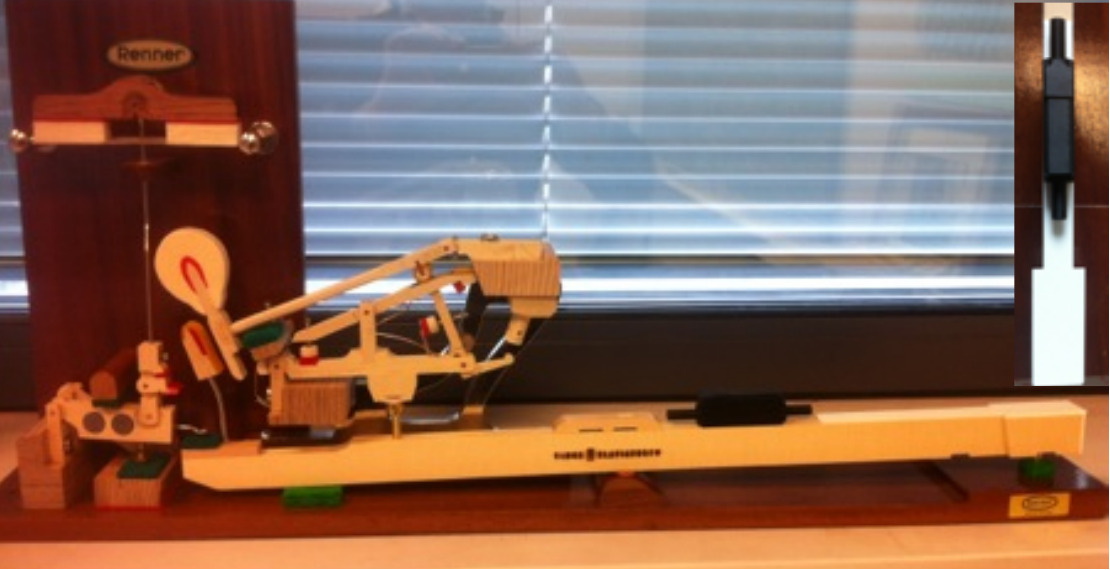
\includegraphics[width=13cm]{MECA_PIANO2.png}\hss}\hfill\null
    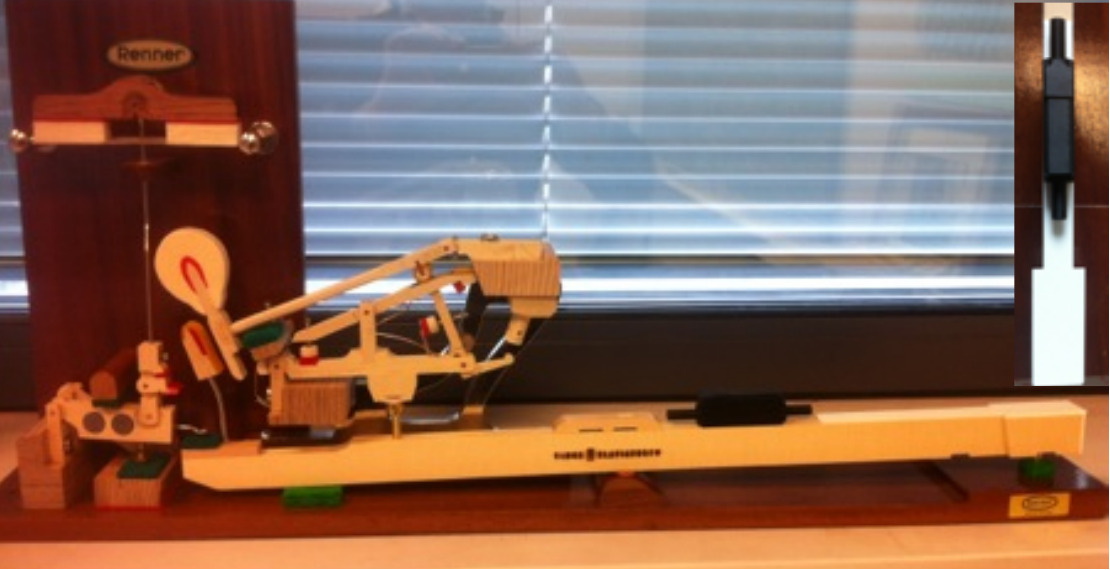
\includegraphics[width=10cm]{MECA_PIANO2.png}
    \caption{Mécanique de Piano}
	\end{figure} 

%Une mécanique de type Renner avec un modèle 3D de l’actuateur linéaire
%envisagé (en noir posé sur la touche) pour donner l’échelle. L’actuateur peut être soit intégré
%dans le sommier en tête de la mécanique sous la cuillère d’étouffoir ou bien positionné à
%l’arrière de celle-ci sur le sommier de cheville. Plusieurs positions seront étudiées. En insert
%une vue de l’actuateur sur la touche qui montre que sa largeur est parfaitement adaptée.

\begin{itemize}
	\item  rapidité : temps de réponse à la milliseconde, vitesse maximum de l’ordre du mètre par
	seconde, accélération de l’ordre de 10 ou 20 g (100 à 200 m/s2 ).

	\item Puissance : force en impulsion de l'ordre de 1kg ou 10N.

	\item encombrement faible: dimension de l'ordre de 1 cm(l) x 1 cm(p) x 5 cm(h).

	\item bruit, inexistant ou négligeable : 10-15 dB à moins de 1m.

	\item précision : positionnement du manche de marteau au dixième (0.1 mm).

	\item fiabilité : durée de vie de milliers d'heures et plus de 10 millions de mouvements.
\end{itemize}

Des moteurs avec ces caractéristiques sont disponibles aujourd’hui et font appel (entre autres) à de puissants aimants miniatures pour les mouvements et à des sondes à effet Hall intégrées pour le positionnement. La figure 5.2 montre un profil de mécanique (c’est a dire la mécanique complète d’une touche individuelle) de la marque Renner, d’autres modèles existent, notamment sur les Steinway, mais leurs caractéristiques essentielles sont semblables. Sur cette même figure, un modèle en impression 3D d’un moteur linéaire de la marque Faulhaber, aux performances mécaniques adaptées à notre problème, est posé sur la touche. On peut voir que ses dimensions sont idéalement adaptées à celles d’un clavier de piano.

L’électronique qui permet la mesure du déplacements des touches (connectée à un capteur de position et/ou un accéléromètre) et qui contrôle l’asservissement doit elle aussi être rapide et précise, si possible intégrée, fiable, puissante et programmable et fera donc appel à de la micro électronique compatible HT (100V) ainsi qu’à des FPGA pour la programmation de l’asservissement et le contrôle du toucher. L’expertise du LPNHE en électronique de pointe et mécanique de précision est un atout déterminant de cette réalisation.

	\begin{figure}[!ht]
    \center
    %\hfill\hbox to 0pt{\hss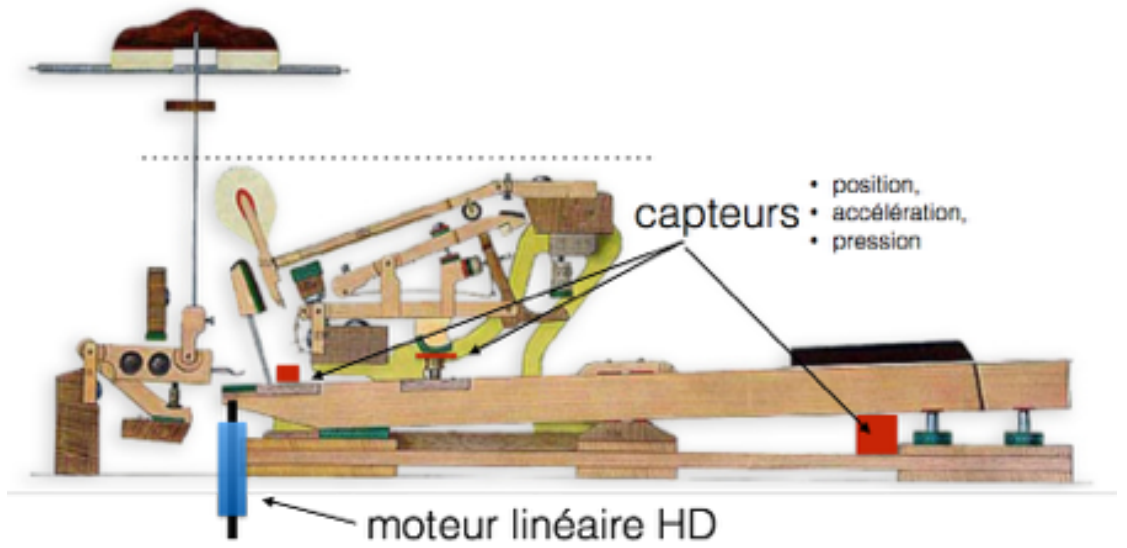
\includegraphics[width=15cm]{MECA_PIANO3.png}\hss}\hfill\null
   	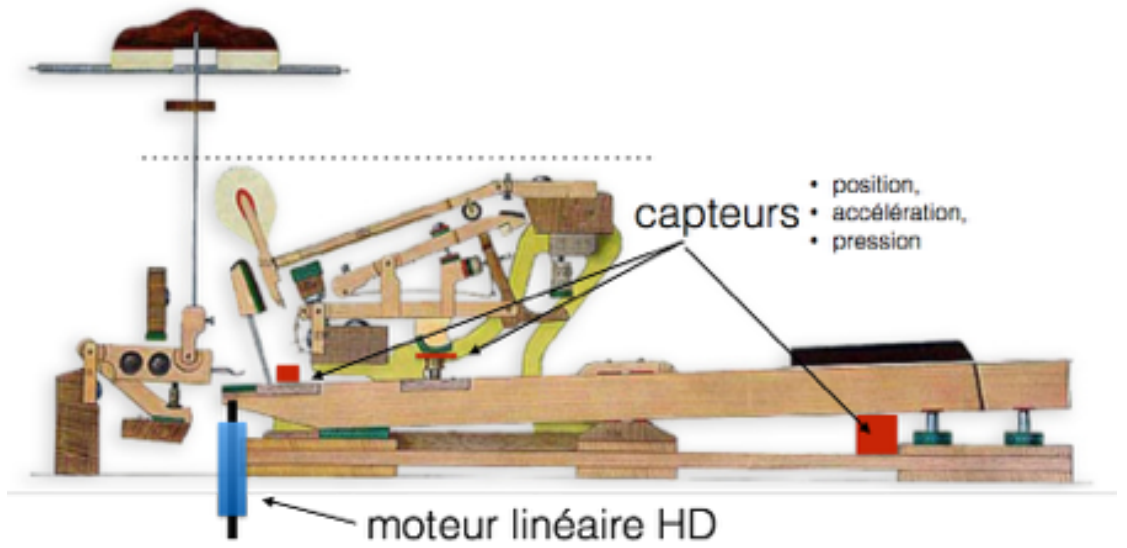
\includegraphics[width=15cm]{MECA_PIANO3.png}
 		\caption{Mécanique de type Renner avec un modèle 3D de l’actuateur linéaire}
	\end{figure}

%Figure 3: une implémentation possible du moteur et des capteurs. Plusieurs types de
%capteurs sont envisageables, accéléromètre sur la touche, capteur de pression entre la
%touche et le pilote, capteur de position sous la touche. Nous étudierons les propriétés de
%chacun et adopterons celui ou la combinaison de ceux qui donnent le meilleur rendu par
%rapport au touché original.

Pour guider les idées, un schéma envisageable d’implémentation est proposé sur la figure 3. L’implémentation optimale nécessite bien-sûr une étude plus approfondie, il s’agit simplement ici de se de fixer les idées. Le moteur et les capteurs de positions sont représentés par les rectangles bleus ou rouges. Sur cette proposition, le rapport (R) entre l’action du moteur et celui du marteau est le même que pour le doigt de l’artiste soit environ 5,5. Les modifications apportées à la mécanique originale sont minimales. Avec un réglage approprié, la sensation
de toucher sera adaptable aux désirs de l’artiste et restera très proche des sensations offertes par la mécanique à répétition et ce même si les marteaux sont lourds car le moteur accompagne en le soutenant le mouvement de la touche mais ne s’y substitue pas totalement.

  \section{Boucle d'asservissement}

La qualité de la boucle de feedback est un point essentiel de notre entreprise. C’est ici que l’expertise de Laurent Bessières donne tout son sens musical au projet. L’asservissement devra d’une part donner aux artistes un confort de jeu digne des meilleures mécaniques avec en plus un équilibrage parfait sur toute l’étendue du clavier. D’autre part, et c’est peut être le plus important, un certain nombre de paramètres de la boucle d’asservissement seront modifiables.

L’échappement et la façon dont il se déroule constituent l’épicentre de l’expressivité. Nous en avons bien conscience et notre intention est bien de le conserver tel quel afin que l’artiste ne soit pas perturbé et puisse donner le meilleur de lui même. Le résultat final dépend également d’un mariage harmonieux entre la mécanique/clavier et l’ensemble harmonique et nous devrons procéder par étape. D’abord assurer que l’apport d’énergie peut se faire de manière quasi transparente pour l’artiste, ensuite exploiter les possibilités offertes par cet apport. Deux axes seront explorés en priorité :

\begin{itemize}
\item  le paramétrage de la courbe de réponse de la mécanique en fonction de l’énergie fournie par l’artiste. On peut élargir ou rétrécir la gamme dynamique et rendre la courbe de réponse non linéaire et des degrés aussi divers qu'imaginables.

\item  la modification physique des éléments de la mécanique, comme le poids et les têtes de marteaux et, en allant plus loin, le point de frappe.
\end{itemize}

Sur tous ces domaines, l’expertise de Laurent Bessières est fondamentale aussi bien pour identifier les paramètres de contrôle que pour qualifier leur gamme et pour la bonne intégration de l’ensemble dans l’instrument. La programmation des fonctionnalités dans le FPGA qui calculera les commandes du moteur à partir des données des capteurs sera elle réalisée par les ingénieurs du LPNHE.

\newpage

  \section{Modélisation}

Thomas Hélie, chercheur à l’IRCAM au Laboratoire des Sciences et Technologies de la Musique et du Son, est spécialiste de la modélisation physique d’instruments de musique. L’un de ses projets de recherche concerne notamment la modélisation, l’asservissement et la commande d’une bouche artificielle robotisé pour le jeux de cuivre. Dans le cadre de notre projet son expertise nous permettra de modéliser les performances de la boucle de feedback en fonction des paramètres mécaniques que nous pouvons ajuster (position de l’actuateur, nombre, nature et position des capteurs). Disposer d’un modèle nous permettra de choisir les configurations les plus prometteuses avant de les réaliser plutôt que d’avoir à toutes les construire et toutes les essayer.

La méthode des systèmes Hamiltionien à ports (Port Hamiltonian System ou PHS) nous permettra de réaliser ces modèles. Cette approche où le système physique étudié est représenté par un ensemble de composants (éléments stockant de l’énergie, éléments dissipatifs, sources externes) reliés par des connexions conservatives (bilan d’énergie ou de puissance) permet une modélisation numérique relativement simple des systèmes complexes. Cette représentation garantie par ailleurs que les lois de conservations sont satisfaites à toutes les interfaces. La modularité du PHS permet d’envisager une complexité graduelle de la modélisation jusqu’à représenter de manière très réaliste l’ensemble touche, chevalet, marteaux ainsi que les commandes d’étouffoir et les ressort de rappel. Dans ce cadre nous nous appuierons également sur les travaux de Xavier Boutillon concernant la modélisation extrêmement réaliste du toucher des mécaniques de piano à queue.

Notons également que l’approche PHS permet d’étudier les réponses non linéaires aux actions extérieures et de calculer les (pré-)contraintes à appliquer sur le signal d’entrée pour obtenir la réponse souhaitée (platitude). Cette approche nous permettra alors de calculer avec précision les paramètres de la boucle d’asservissement. Là encore l’expertise de Thomas Hélie nous permettra d’élaborer ces modèles de manière efficace et optimale.



%--------------------------------------------------------------------------------------
%
% Caractérisation technique du projet
% objectifs
% déroulement prévu
%
%--------------------------------------------------------------------------------------
\part{Projet "CHAMP", étude et caractérisation}

	\chapter{Introduction au projet}
	
	\section{Synthèse et objectif du projet}
	
	Comme dit précédemment, le projet "CHAMP" est né de la rencontre de personne et de la mise en commun de savoir provenant d'univers variés, à savoir, 
	
	le milieu scientifique, au travers du LPNHE (laboratoire de physique nucléaire et des hautes énergies), représenté par Antoine LETESSIER SELVON, physicien des hautes énergies et directeur de recherche, Hervé LEBBOLO, ingénieurs de recherche, et enfin,  Philippe REPAIN, mécanicien chef d'atelier.
	
	le milieu musical artisanal, représenté par Laurent Bessières détenteur du prestigieux titre d'Académicien Steinway.
	De plus, depuis l'inauguration de la philharmonie de Paris en janvier 2015, Laurent en est l'accordeur référant de la philharmonie. Enfin, il travaille également avec d'autres prestigieuses salles, comme Steinway and Sons France, régie Pianos, la Salle Pleyel, la Salle Cortot ou le Studio de la Grande Armée qui font régulièrement appel à ses services.	
	
	Au travers de cette rencontre, plus que de vouloir proposer un piano de concert connecté, nouvelle génération, le projet prend racine au travers d'une idée simple mais précise, élargir les possibilités de l'instrument en n'en modifiant la mécanique interne, tout en conservant inchangé, l'expérience utilisateur.
	Pour cela, décision fut prise de s'appuyer sur les techniques et les technologies modernes afin de faire évoluer l'instrument, le piano.
	
	Ainsi, sans altérer l'expérience utilisateur, ce rapport étroit entre le musicien et son l'instrument, représentant de nombreuses années de pratique, les artistes auront à disposition des nouveaux moyens d'expression, offrant de nouvelles possibilités de jeux.
	
	\newpage
	
		\subsection{Un nouveau moyen d'expression}
		
		Afin de proposer de nouveaux moyens d'expression, il a tout d'abord fallu identifier au sein du piano, l'élément étant la source de l'identité "musicale" ; des harmoniques de l'instrument. C'est en modifiant, en retravaillant la mécanique autour de cette pièce, que nous pourrons apporter de nouvelles expériences de jeux.
		
		Grâce aux articles de spécialistes, précédemment cité, le marteau, plus que la touche ou le chevalet, apparaît comme éléments ayant l'incidence majeure sur l'harmonisation de l'instrument, au travers de son poids.
		
		L'intégration de nouvelles technologies au sein du projet, aura donc pour but de permettre une variation du poid du marteau, afin de fournir une large palette d'harmonique au musicien, qui n'aura plus qu'à laisser court à son imagination et à sa technique afin de tiret le meilleur de l'instrument lors de compositions musicales.
	
	\section{Rôle au sein du projet}	
	
	Recruté en tant que stagiaire, assistant ingénieurs, sur ce projet. Mon rôle fut prendre connaissance du projet, étudier l'état de l'art quant aux recherches déjà effectuées et d'avoir un regard critique sur ces dernières. Être force de propositions sur l'intégration de solutions techniques, sur des problématiques directes, ainsi que sur des fonctionnalités futures; les développer et enfin mener leurs intégrations au sein du projet.
	
	Avant mon arrivée, l'équipe en place avait déjà commencé à travailler sur une preuve de concept, s'appuyant sur une base d'électronique analogique, cœur de métier du laboratoire. Mais suite à mon arrivée, nous avons ensemble, redéfini le cadre du projet, afin de garder les idées et concepts testés et approuvés lors de cette première approche, tout en faisant évoluer le projet en basculant sur une base orientée électronique numérique, système embarqué.
	
	De plus, j'ai eu pour rôle de faire part de l'avancement de mon travail, ainsi que mes observations autour du projet, à mon maitre de stage et directeur de recherche, lors de réunions durant lesquels nous définissions ensemble l'avancement des différentes étapes et discutions de nouvelle(s) fonctionnalité(s) pouvant être intégré au projet.
	
	Enfin, j'ai pu être force de proposition quant aux futur fonctionnalités du projet, ce dernier étant une preuve de faisabilité, il dispose d'un cahier des charges au contour assez vague, induisant une plus grande liberté d'esprit, quant aux innovations pouvant être apportées.	
	
	
	\chapter{Les travaux menés}
	
	Comme expliqué précédemment, suite à mon arrivée au LPNHE, j'ai commencé par prendre connaissance de l'architecture globale du projet (figure ci-dessous) et des concepts et idées qui avaient déjà étés pensé et proposé, ainsi que des diverses solutions techniques à l'étude concernant des choix de composants.
	
	J'ai ainsi commencé par travailler sur le développement de la chaine de contrôle la plus simple pouvant être mise en place, afin d'éprouver les choix et solutions techniques retenues.
	Cette chaine, représentant l'action d'une touche du piano, ce comporte comme suivant: Un accéléromètre mesurant l'accélération du marteau, (dû à une force appliquée sur une touche du piano) communiquant avec une carte programmable munie d'un FPGA, appliquant un filtre numérique sur les données reçu, pour ensuite les faire parvenir à un convertisseur numérique analogique (CAN), assurant la transmission des données à notre contrôleur moteur.\newline
	
	\begin{figure}[!ht]
    \center
    %\hfill\hbox to 0pt{\hss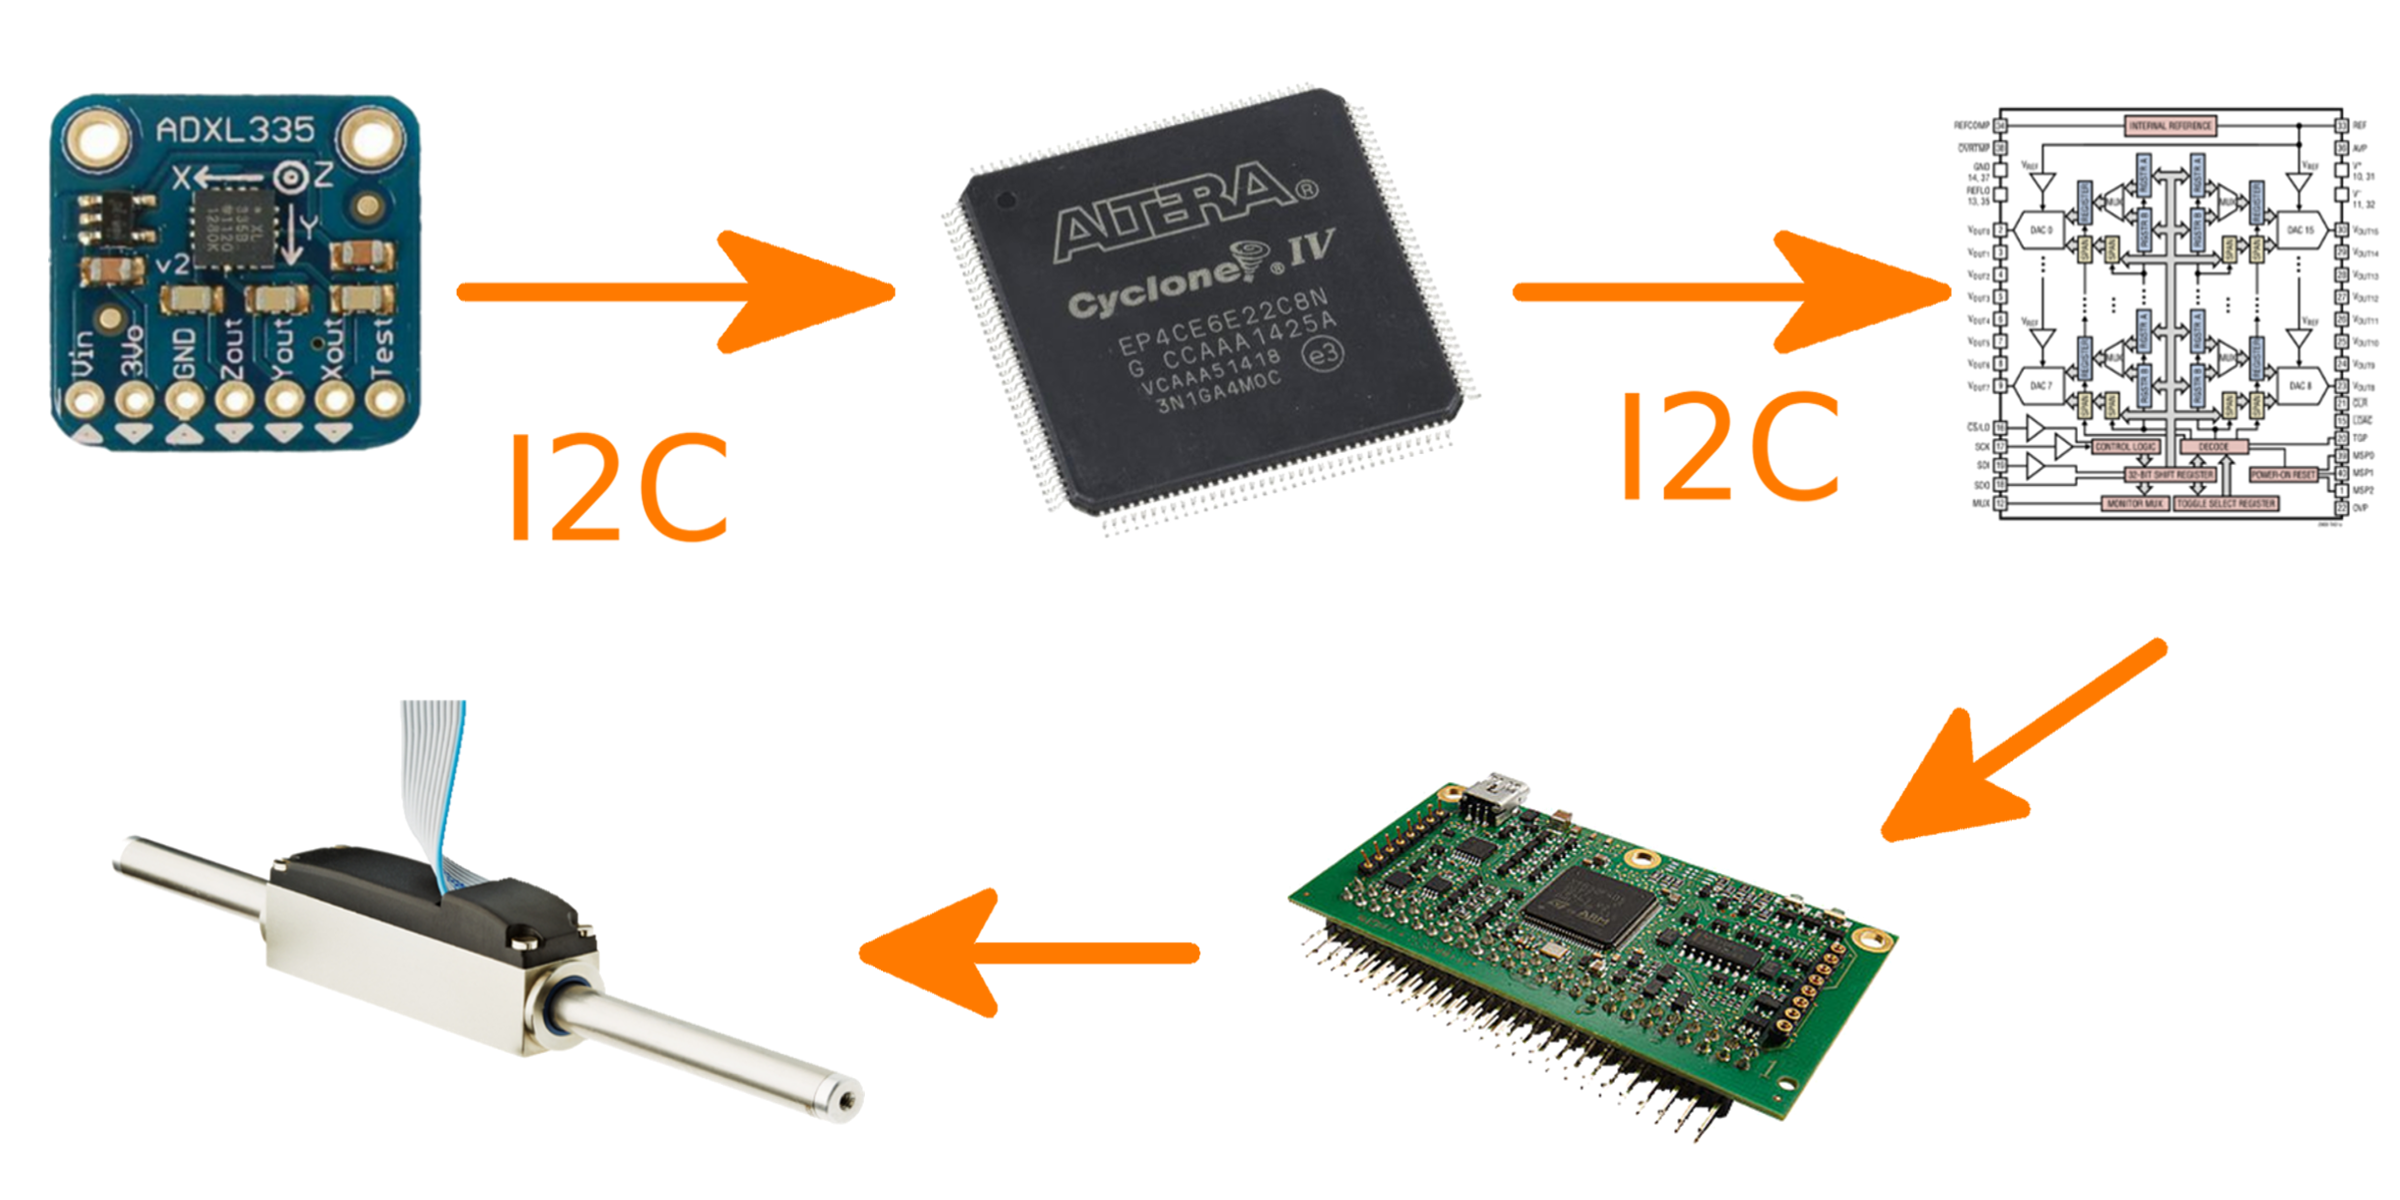
\includegraphics[width=17cm]{CH.png}\hss}\hfill\null
  	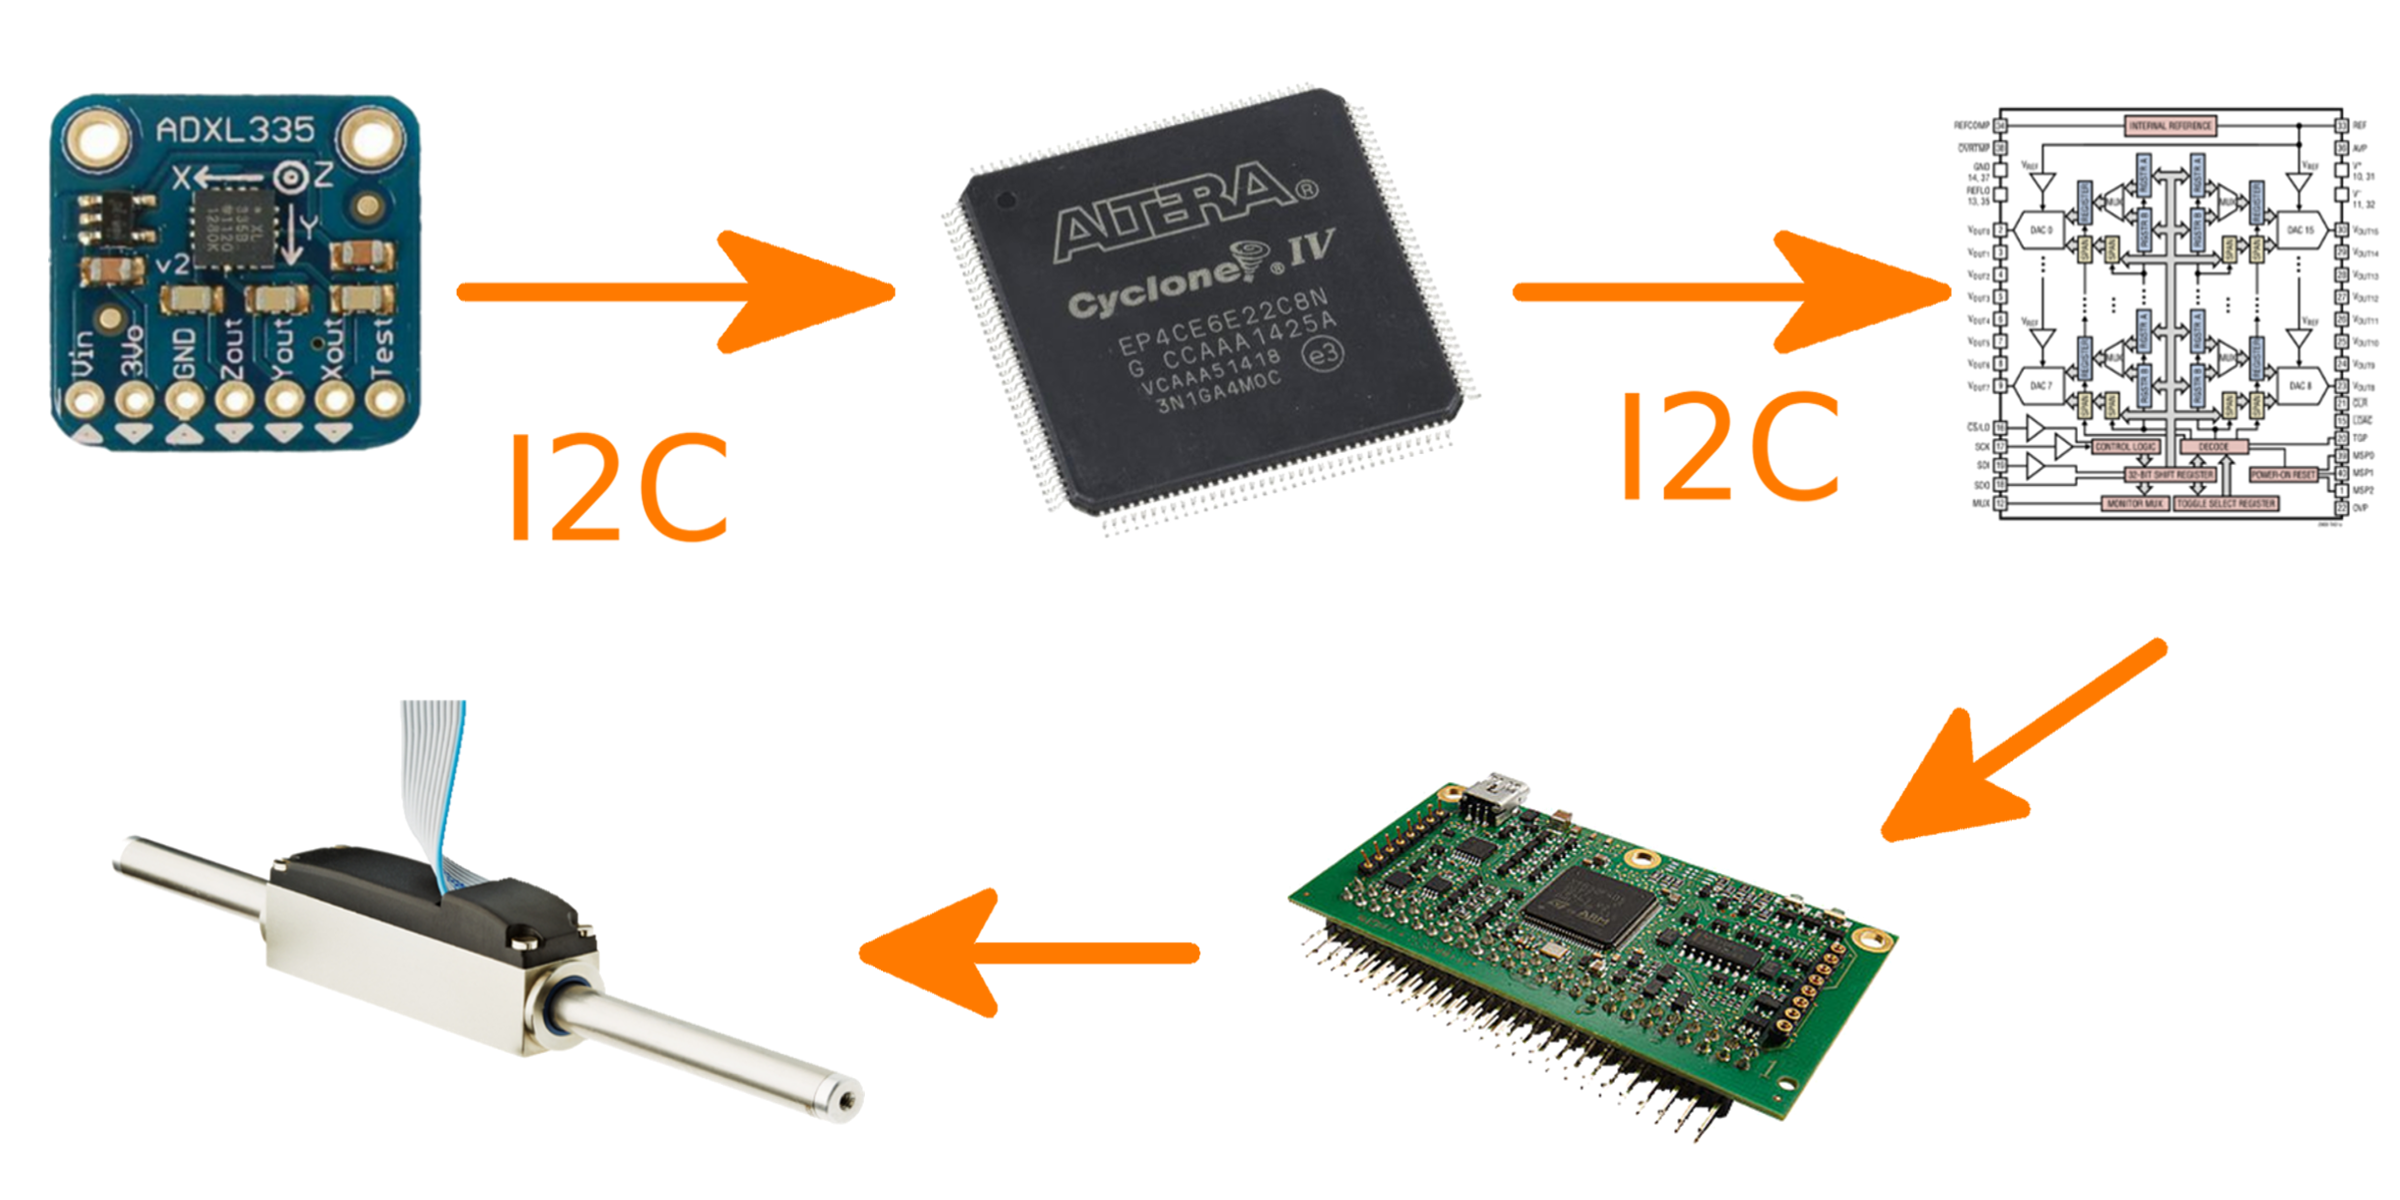
\includegraphics[width=17cm]{CH.png}
    \caption{Chaine de contôle d'une touche de Piano}
	\end{figure}	
	
	Ainsi, la toute première tâche réalisée fut de mener une étude de cas entre les deux bus de communication à disposition, le bus I2C et le bus SPI, afin de déterminer lequel serait le plus adapter à notre projet.
	
	Cette étude de cas, m'a par la suite conduit à éprouver un "hacking" sur notre accéléromètre. Notre choix de bus de communication induisant un grand notre de câble de branchement, nous souhaitions en faire diminuer le nombre.
	
	La suite logique à cette étape, fut d'étudier le bus de communication sélectionné, afin de l'instancier au sein du projet, en se basant sur le langage VHDL. Ce bus de communication étant présent en deux endroits de la chaine, entre l'accéléromètre et la carte programmable FPGA et entre cette dernière et notre convertisseur numérique analogique, notre intégration devait répondre aux spécificités des deux cas d'utilisation, afin de ne pas faire doublons dans la mise en place de solution, ainsi que dans les potentielles sources d'erreurs.
	
	Puis, après avoir éprouvé l'échange de données, entre les différentes entités, un filtrage numérique fut intégré à notre carte programmable. Ce filtrage ayant pour but de mettre en place un asservissement numérique sur le contrôle des moteurs.
	
%	Par la suite, nous avons choisi de mettre en place une solution de monitoring, afin de pouvoir visualiser nos données échangés ,en temps réel sur un ordinateur.

	Par la suite, différents prototypes de cartes électroniques (PCB) on dut être réalisé et réévaluer au long su projet, afin de répondre aux impératifs d'intégration matérielle au sein du piano.
	
	Enfin, une étude de "rétro-engineering", fut menée en salle de test sur des éléments électroniques tiers, fournie par notre partenaire technique, l'entreprise "Faulhaber", afin d'en vérifier le bon fonctionnement, mais également d'en valider le comportement vis-à-vis de l'utilisation souhaitée.
	
	Mais comme expliqué en ce début de partie, ce module, illustré ci-dessus, n'est que d'un douzième du prototype final; ne permettant la récupération et le traitement que d'un seul accéléromètre à la fois et donc, d'une seule touche à la fois.
	
	La maquette à réaliser étant composé de 12 touches, il nous faudra par la suite, généraliser notre module afin de récupérer et traiter les informations de nos 12 touches, de manière parallèle.
	Ce travail étant un peu plus complexe que le module précédemment présenté, il demande une refonte d'une partie de la chaine, vis-à-vis de l'échange de données entre la carte programmable (FPGA) et le convertisseur numérique analogique (CNA).
	
	\chapter{Planning}

	Ci-dessous sont présentés sous forme de diagrammes de Gant, le calendrier prévisionnel ainsi que le calendrier réel du travail réalisé tout au long su stage.
	On y retrouve un descriptif complet et détaillé des différentes tâches réalisées.
	
	On peut observer sur le calendrier réel, que les phases de test, de débug, n'avaient pas été prises en compte lors de l'établissement du calendrier prévisionnel.
	À l'avenir, ces tâches ne seront plus négligé, étant donné le caractère important de celles-ci, du fait de leur capacité à bloquer l'avancement d'un projet, et induire des retards plus ou moins importants.
	
	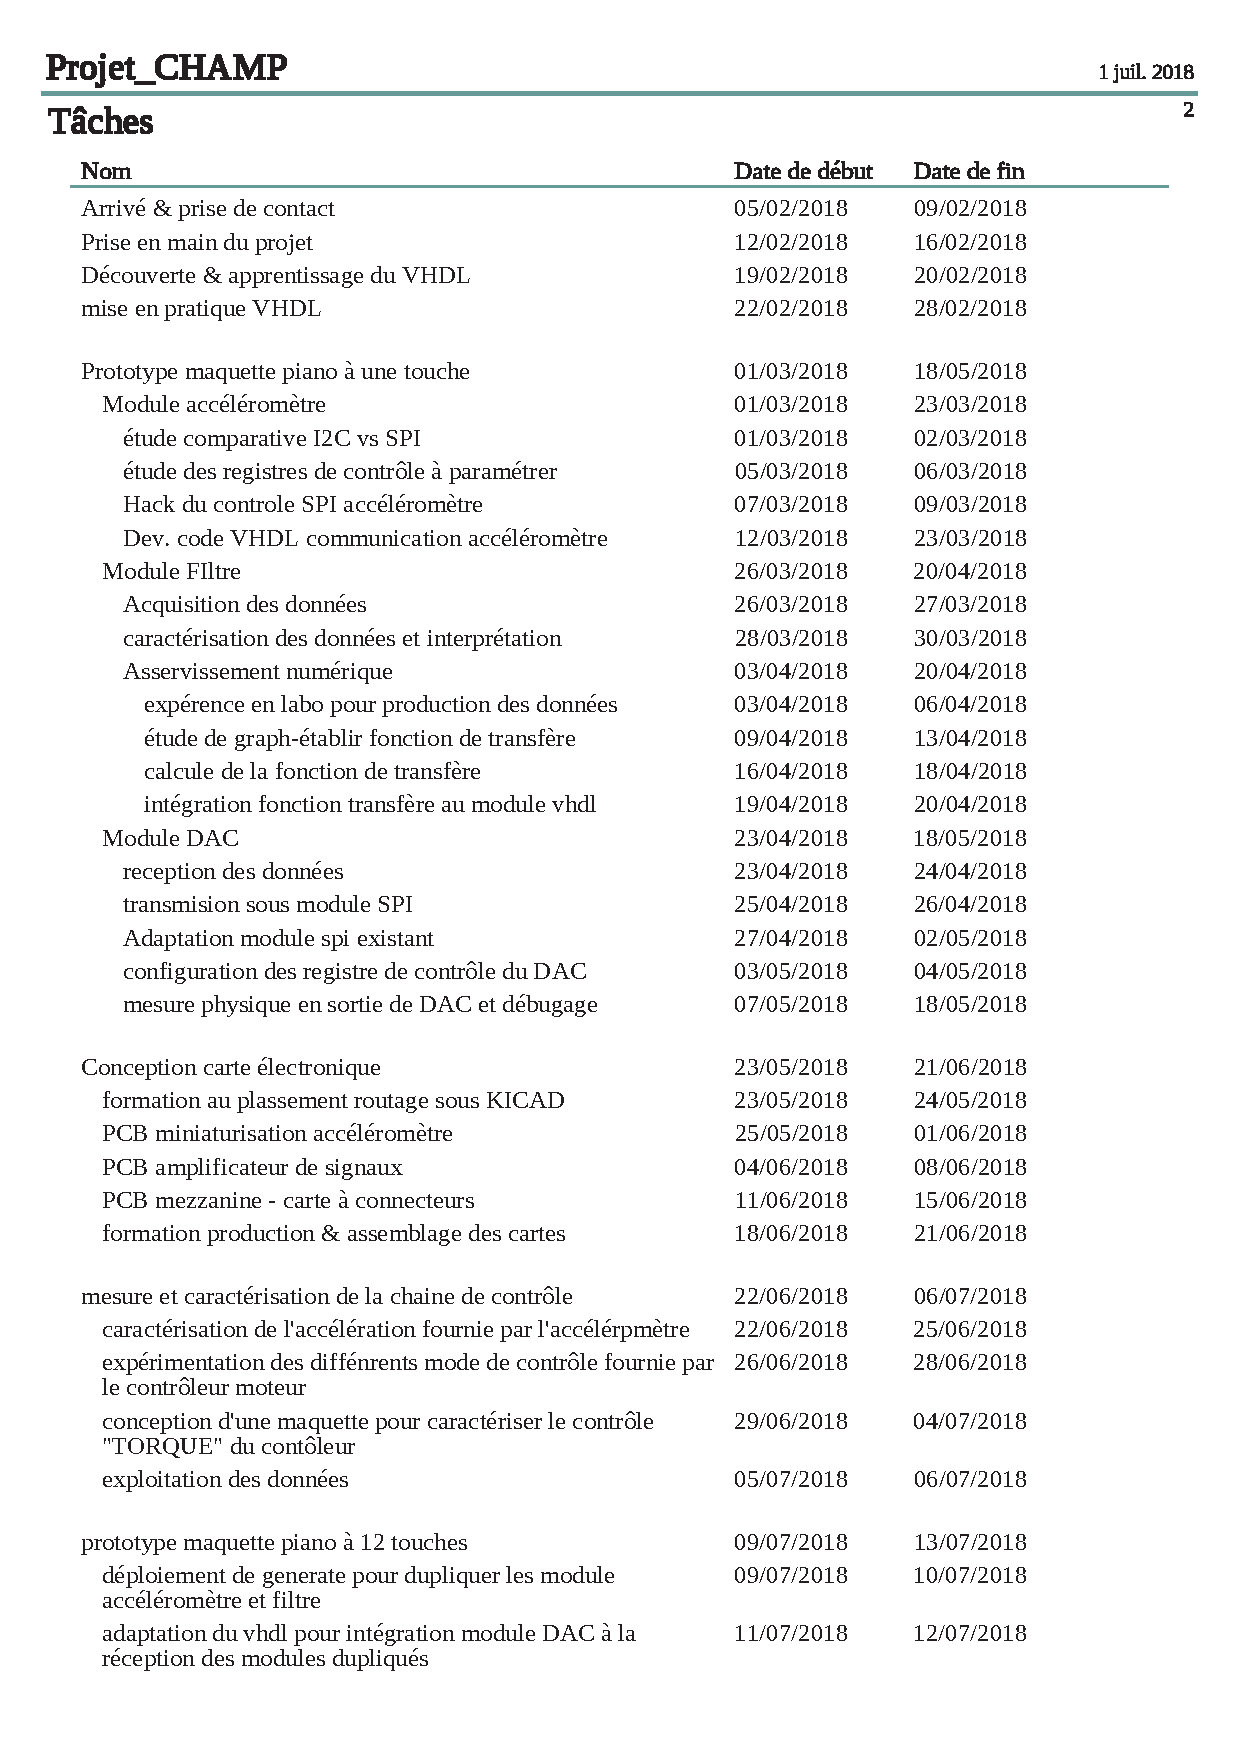
\includepdf[scale=1, pages=-]{calendrier_Previsionnel_defA}
	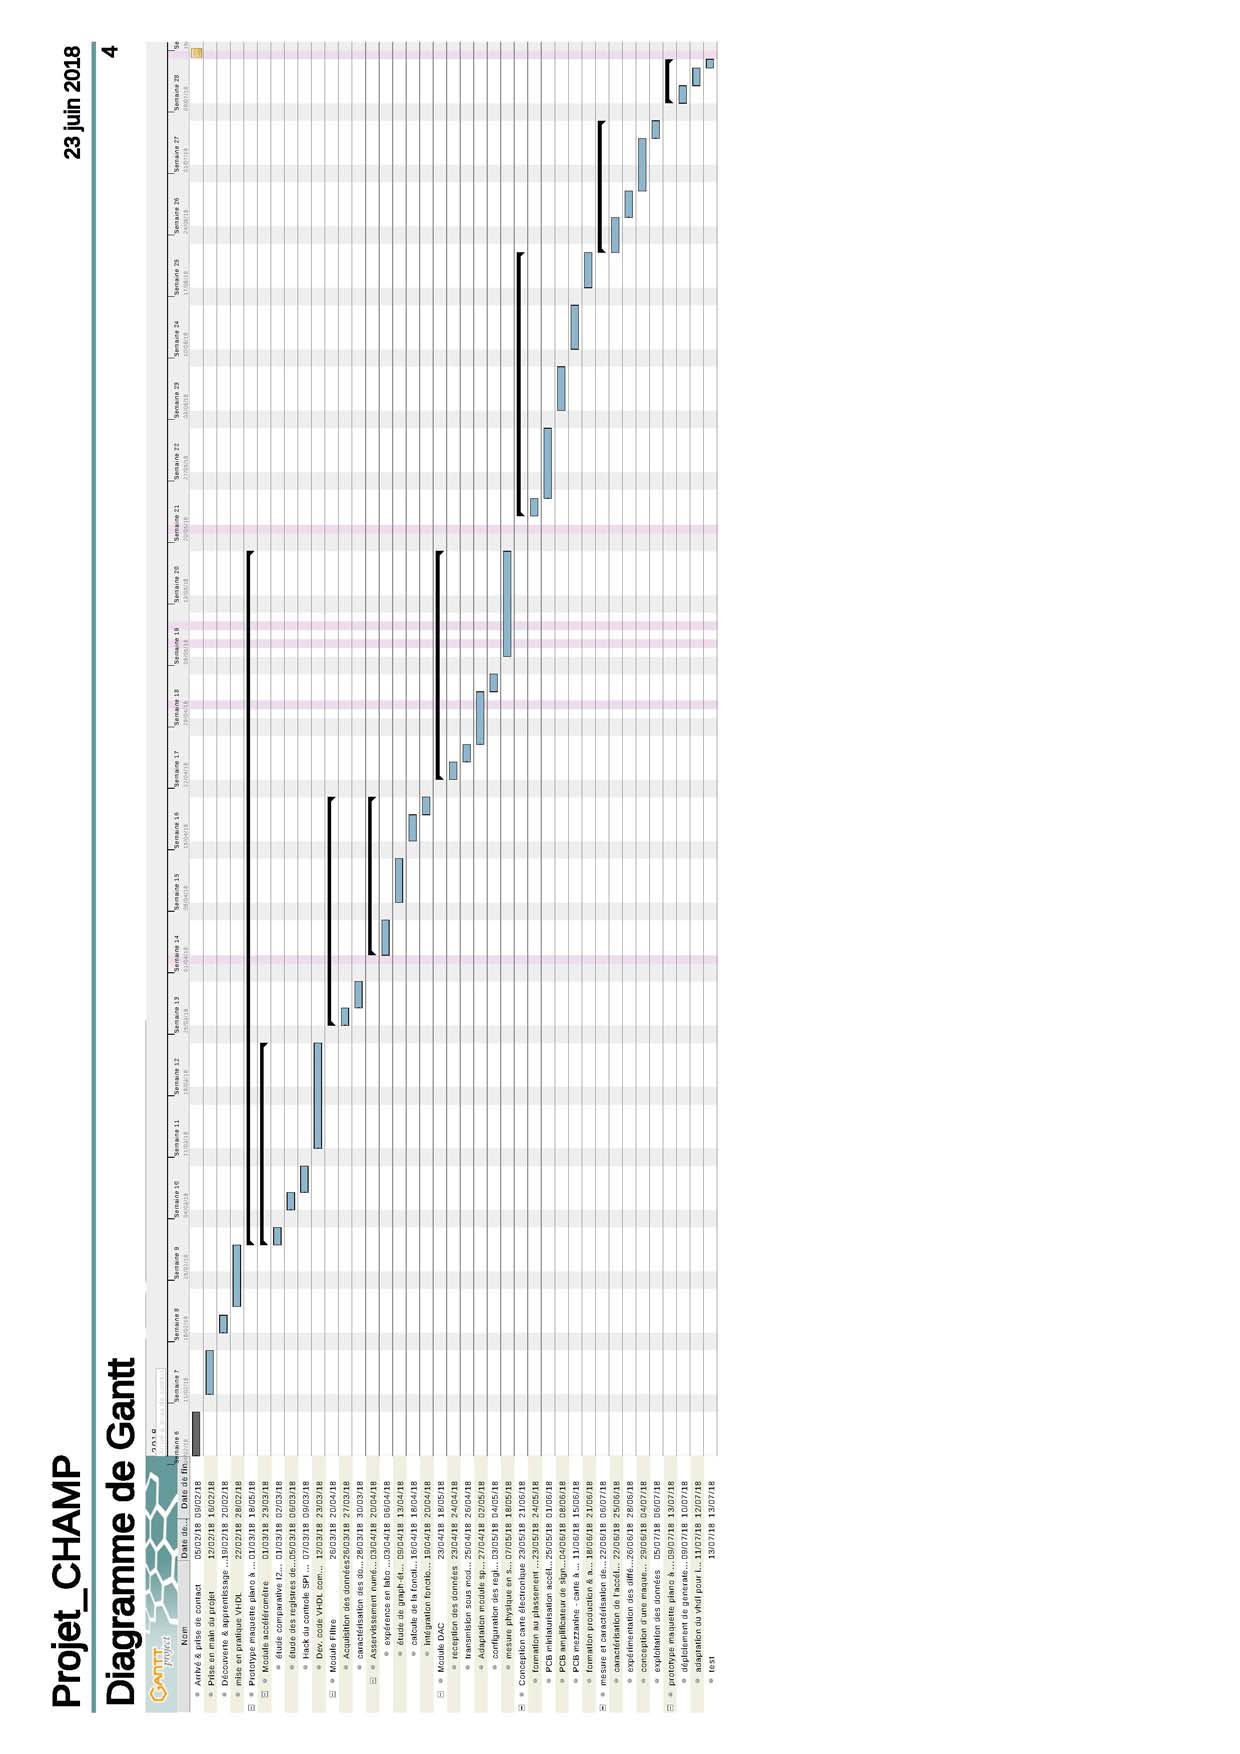
\includepdf[scale=1, pages=-]{calendrier_Previsionnel_defB}
	
	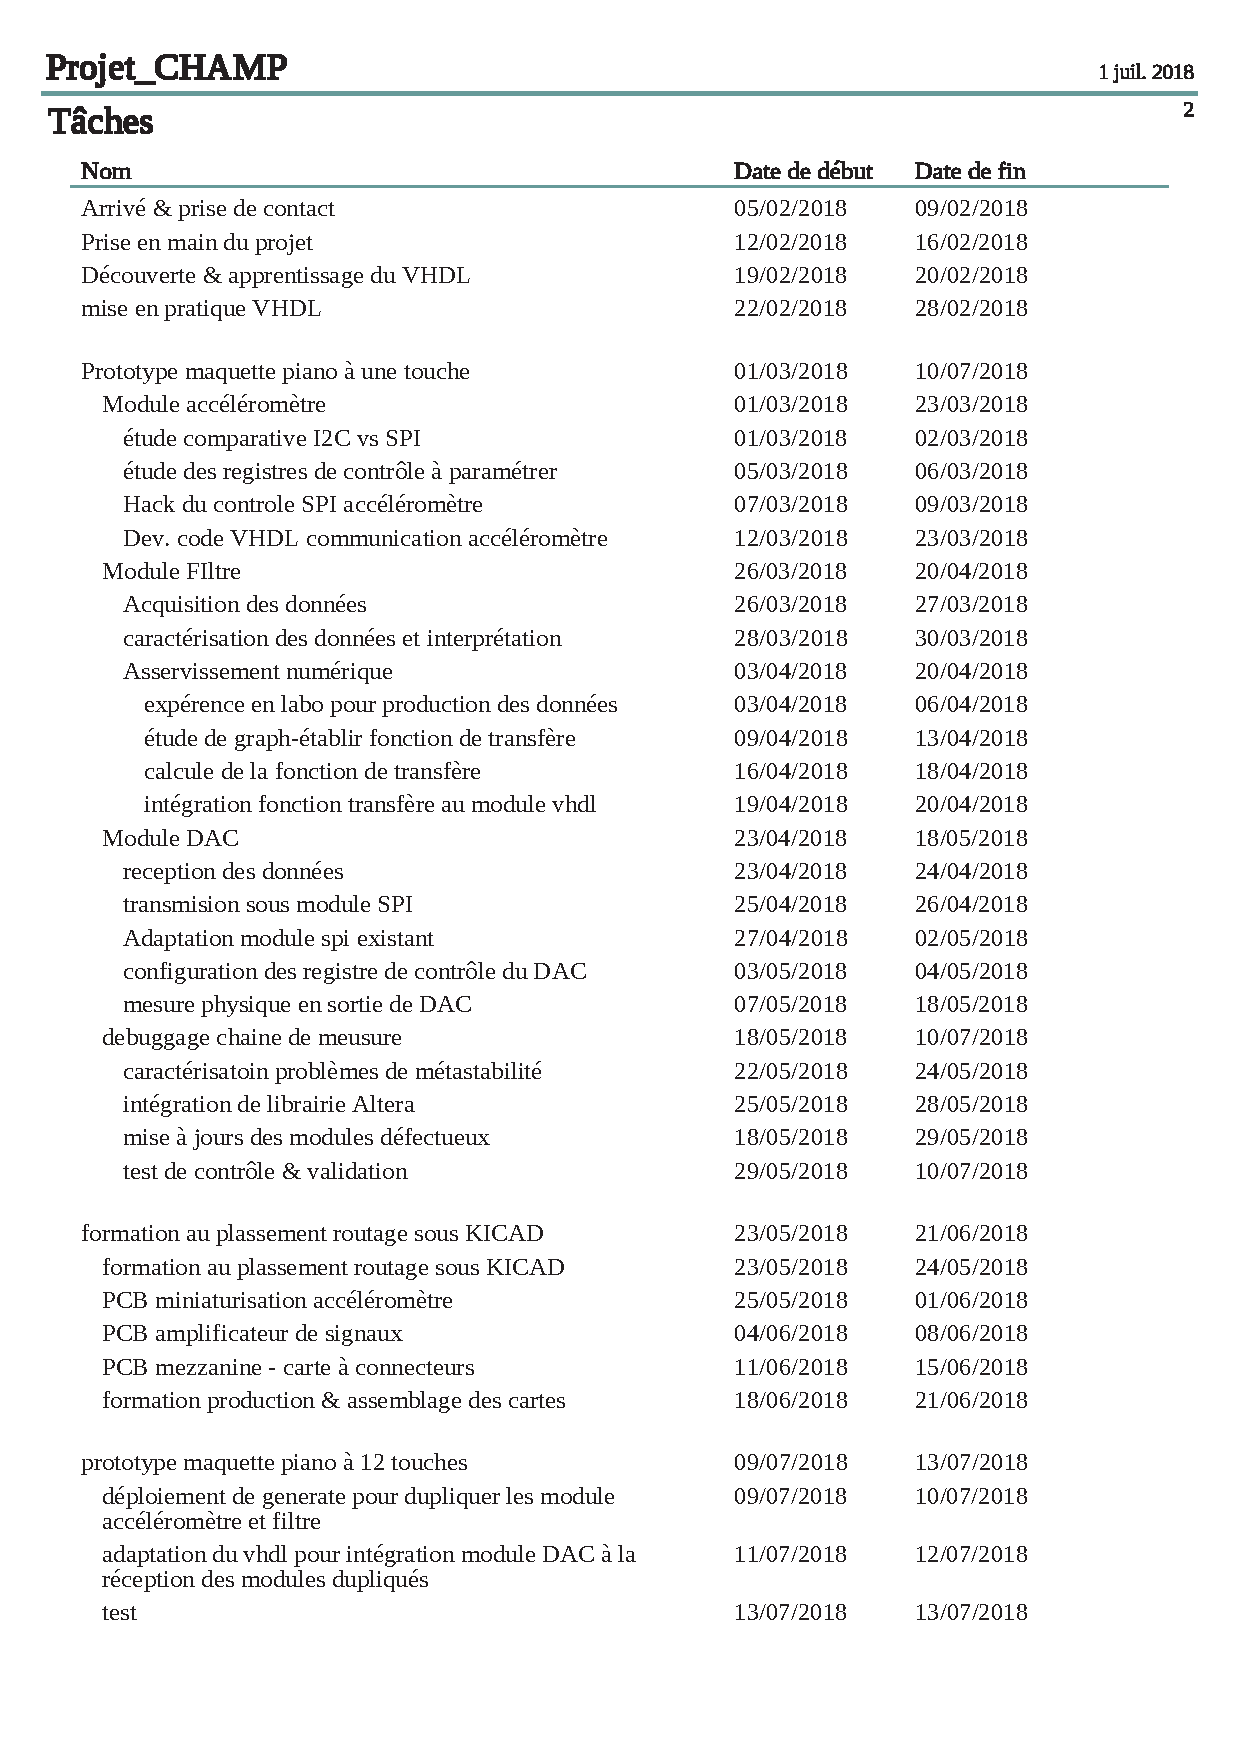
\includepdf[scale=1, pages=-]{calendrier_reel_defA}
	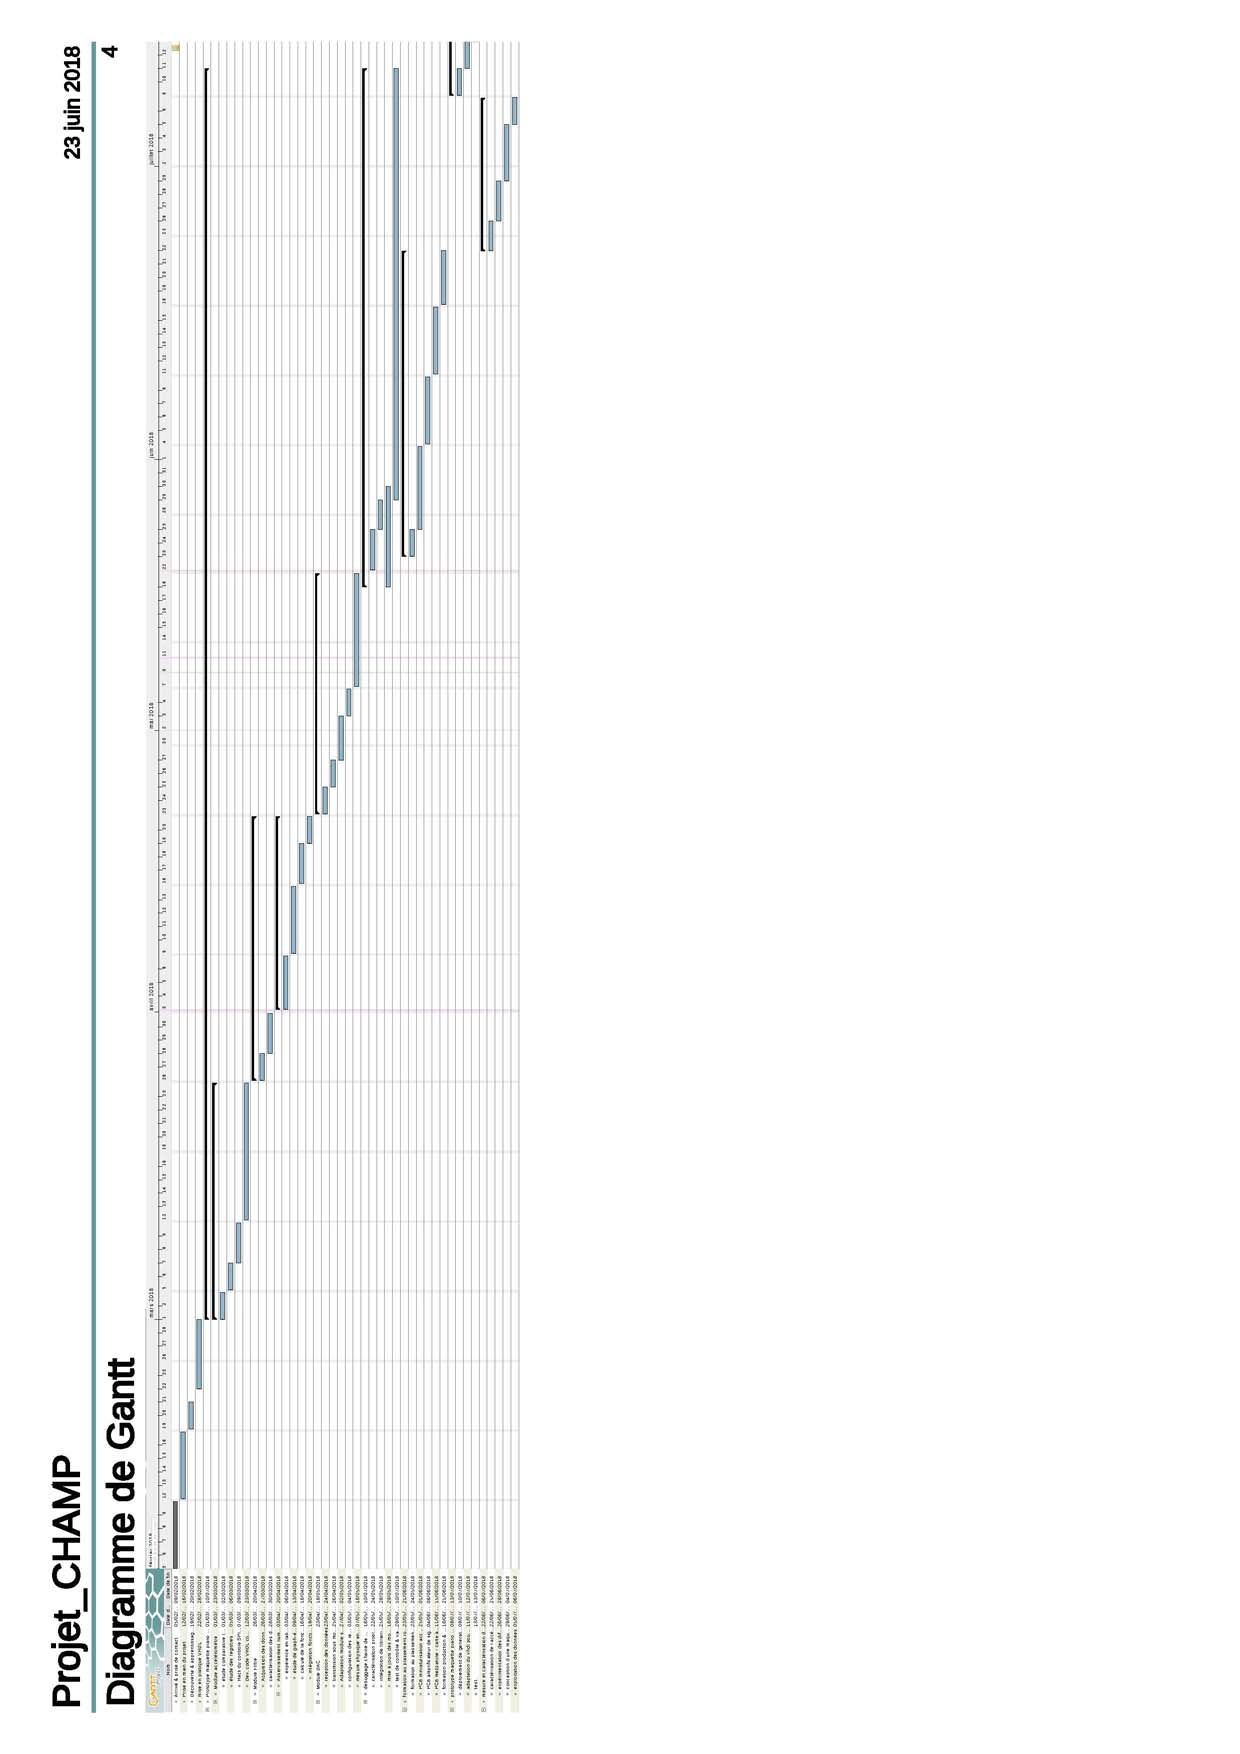
\includepdf[scale=1, pages=-]{calendrier_reel_defB}	
	
	
	
	
%--------------------------------------------------------------------------------------
%
%	Présentation et Détail des travaux Réalisés durant le stage
%
%--------------------------------------------------------------------------------------

	
	\part{Travaux et réalisation}	
	
	\chapter{Réalisation de la chaine de contôle}
	
	
	
	
	\chapter{Asservissement et caractérisation}
	
	Lors de la précédente partie, nous avons abordé l'ensemble des aspects qui nous ont permis de mettre au point notre chaine de contrôle; en partant des données fournies par notre accéléromètre, leurs réceptions et leurs traitements au sein de notre carte programmable (FPGA), jusqu'à leur envoi et leur réception par le Convertisseur Numérique Analogique, permettant le contrôle du contrôleur moteur, en lui transmettant des consignes de fonctionnement.
	
	Lors de cette partie, nous allons nous concentrer sur la mise au point de l'asservissement numérique, élément indispensable, devant prendre place au sein du filtre numérique de notre carte programmable FPGA.
	
	L'asservissement numérique est un processus en plusieurs étapes, consistant à piloter un système tiers, en mesurant périodiquement des valeurs de consigne, fournies par un système de capteurs, dans notre cas, un accéléromètre. 
	Par la suite, ces données sont traitées par notre calculateur, mais étant donné le mode de traitement des informations imposé par notre calculateur est de nature numérique et cadencé dans le temps de façon périodique grâce à une horloge; les informations en entrée, provenant de nos capteurs, sont donc des grandeurs discrètes.
	
	Les différentes étapes que l'on retrouve,  générique à tout système asservi sont les suivantes:
	
	\begin{itemize}
		\item l'échantillonnage d'un signal continu
			Cette opération consiste à relever les informations prises par un signal continu à intervalles de temps
			régulier, appelée période d'échantillonnage. On parle alors de signal échantillonné, signifiant que le
			calculateur ne tiendra compte que des valeurs prises par le calculateur aux instants d'échantillonnage.
			
		\item La conversion d'un signal analogique en un signal numérique
			Il s'agit de convertir la valeur prise par un signal analogique à l'instant d'échantillonnage en une
			valeur numérique, afin qu'elle puisse être traitée par le calculateur. Un tel signal peut, par exemple, 
			provenir d'un capteur. On parlera alors de signal de mesure.
			 
		\item La conversion d'un signal numérique en un signal analogique
			Cette opération consiste à transformer le signal numérique issu du calculateur à l'instant 
			d'échantillonnage (on parlera de signal numérique de commande), en signal analogique de commande 
			existant sur toute la période d'échantillonnage, l'objectif étant de commander le système physique.
			
		\item  La synthèse d'un algorithme de calcul
			Il s'agit d'établir une loi d'évolution du signal de commande numérique en fonction des signaux de mesure
			et de référence, également numériques, afin de permettre au système asservi de satisfaire un cahier des
			charges. Cette fonction est appelée correcteur numérique ou encore loi de commande numérique. Elle a pour
			objectif de déterminer la valeur du signal numérique de commande à un instant d'échantillonnage, à partir 
			d'un algorithme de commande, de mesure et de référence.
	\end{itemize}
	
	Ainsi, l'on peut résumer sous forme de schéma bloque une structure classique d'asservissement numérique comme suivant:
	
	\begin{figure}[!ht]
    \center
    %\hfill\hbox to 0pt{\hss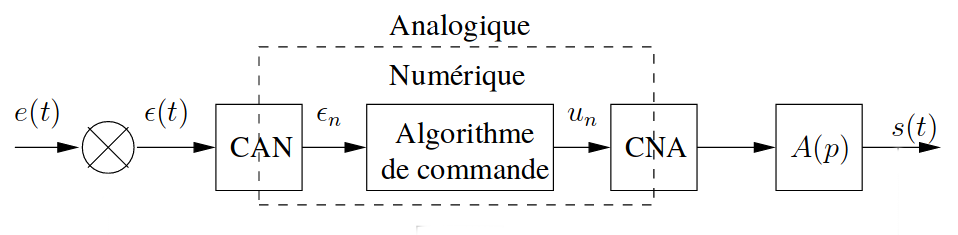
\includegraphics[width=17cm]{Assert_1.png}\hss}\hfill\null
  	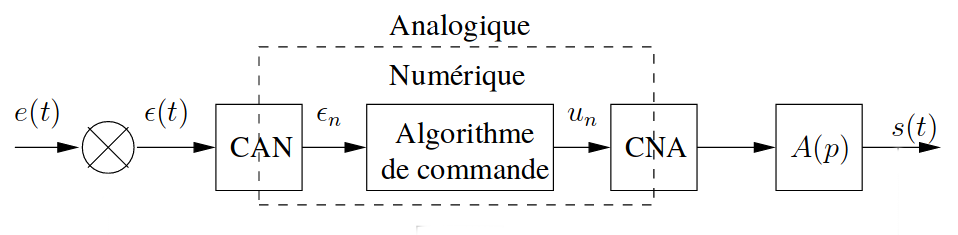
\includegraphics[width=17cm]{Assert_1.png}
    \caption{Structure classique d'asservissement numérique}
	\end{figure}	
	
	De plus, l'asservissement numérique de notre projet implique la caractérisation de la fonction de transfère de notre système dans son ensemble.
	Ainsi, afin de déterminer notre fonction de transfère, seront présenté les différents protocoles et les différentes manipulations effectués sur notre banc de test.

	\section{Asservissement du projet Champ}
	
		Au sein de notre projet, notre asservissement va reprendre les différentes étapes présentés ci-dessus. Ainsi, concernant l'échantillonnage d'un signal continu, cette étape est réalisée au sein de notre accéléromètre étant donné que ce dernier nous fournit un signal échantillonné à une fréquence de 1 KHz (Période d'une milliseconde). Notre accéléromètre disposant d'un convertisseur analogique numérique intégré sur chaque axe, c'est au sein de ce dernier que s'effectue l'opération d'échantillonnage du signal continue.
		
		Par la suite, c'est au sein de notre carte programmable FPGA que s'effectue la phase de traitement sur notre signal discret. C'est au sein de notre filtre numérique que va être appliqué l'algorithme de synthèse sur les mesures en provenance de l'accéléromètre, afin d'asservir le système contrôlé, selon le cahier des charges.
				
		Enfin, la fonction de conversion de notre signal numérique en un signal analogique est assurée par le convertisseur numérique analogique (CNA) ayant pour rôle de fournir une commande au contrôleur moteur, existant sur toute la période d'échantillonnage, afin de commander notre système physique.
		
		Comme précédemment, on peut résumer l'asservissement mis en place pour le projet CHAMP, sous la forme d'un schéma bloc, comme suivant:
		
	\begin{figure}[!ht]
    \center
    %\hfill\hbox to 0pt{\hss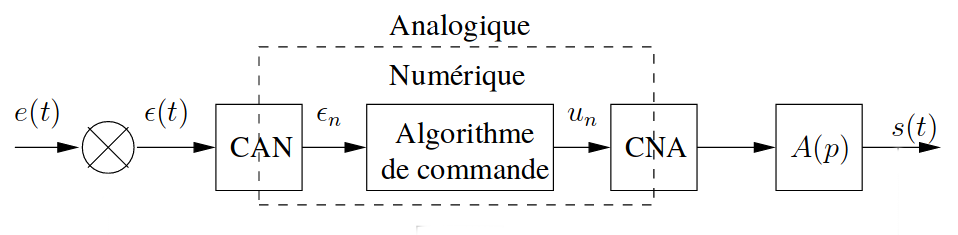
\includegraphics[width=17cm]{Assert_1.png}\hss}\hfill\null
  	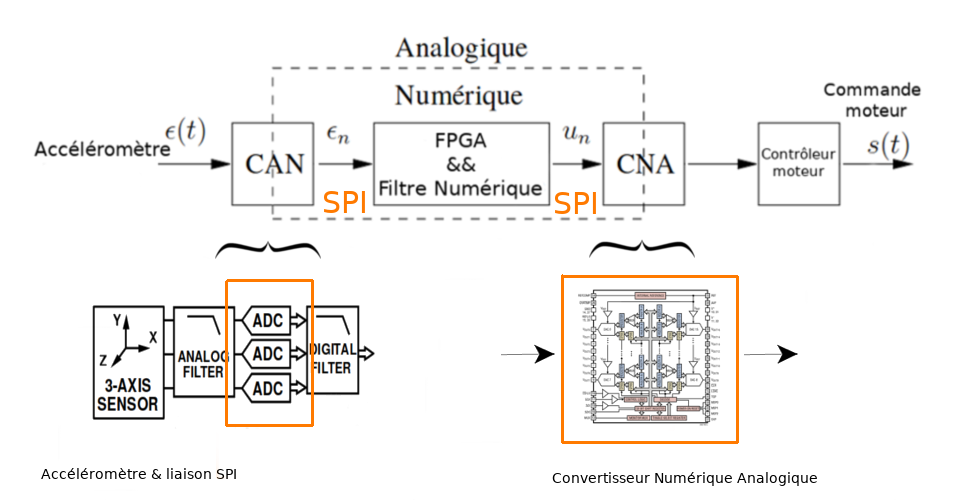
\includegraphics[width=17cm]{Assert_2.png}
    \caption{Asservissement numérique du projet CHAMP}
	\end{figure}	
		
		
	\section{Fonction de transfère}
	
		La fonction de transfère de notre système correspond à l'algorithme, appliqué sur nos données (discrètes) au sein du filtre. Une fois les données sorties de cet algorithme, les données sont aptes à piloter notre système tiers comme nous le souhaitons.
		
		Une fonction de transfère est le modèle mathématique de la relation entre la sortie et l'entrée de notre système ; le plus souvent cette fonction étant invariante en fonction des paramètres d'entrer.
		Du point de vue d'une approche physique, la fonction de transfère caractérise la dynamique du système; elle ne dépend que de ses caractéristiques physiques. 
		Ainsi, un système sera décrit par sa fonction de transfert est représenté comme suivant:

	\begin{figure}[!ht]
    \center
    %\hfill\hbox to 0pt{\hss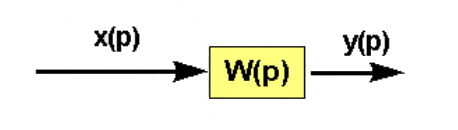
\includegraphics[width=17cm]{transf1.png}\hss}\hfill\null
  	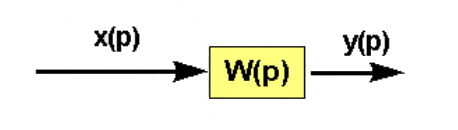
\includegraphics[width=5cm]{transf1.png}
    \caption{Modèle quelquonque}
	\end{figure}
	
	Nous aurons donc la fonction de transfère suivante : W(p) = Y(p) / x(p).
	
	\newpage
	
	\section{Première manipulation}
	
		\subsection{Introduction}
	
		À travers cette première manipulation, nous avons cherché à déterminer la fonction de transfère de notre modèle, en visualisant à l'aide d'un graphique, les données fournies en entrée du système (provenant du DAC), ainsi que les données en sortie de notre modèle (une fois traitées par le contrôleur moteur).
		En procédant ainsi, nous allons pouvoir observer et comparer l'évolution de nos courbes en fonction du temps et ainsi déterminer si ces dernières évoluent selon le même schéma, ou si le traitement des données par le contrôleur moteur induit un retard au sein du système.
		
	On retrouve ci-dessous, le schéma bloc de la première manipulation réalisée.
		
	\begin{figure}[!ht]
    \center
    %\hfill\hbox to 0pt{\hss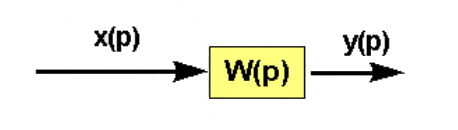
\includegraphics[width=17cm]{transf1.png}\hss}\hfill\null
  	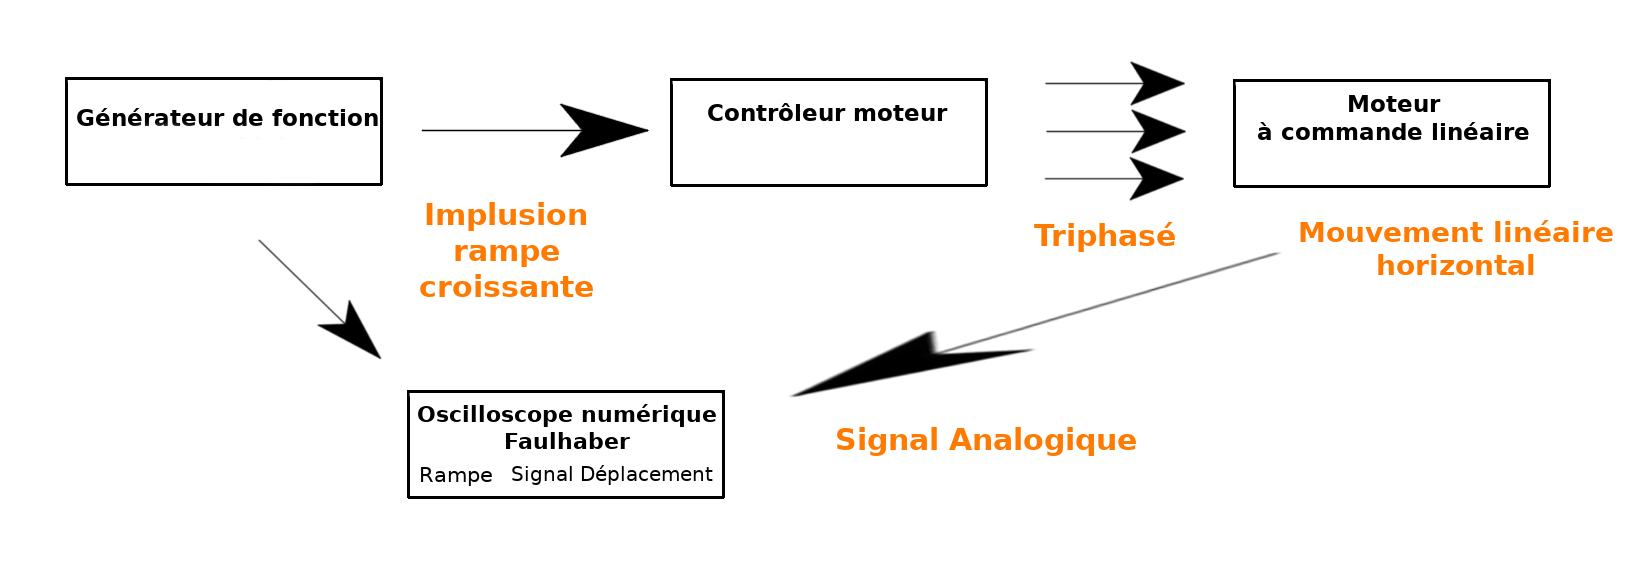
\includegraphics[width=18cm]{manip1.png}
    \caption{Schéma bloc - Première manipulation}
	\end{figure}	
		
		Comme illustré ci-dessus, nous utilisons un générateur de fonction afin de transmettre une impulsion au contrôleur moteur, sous la forme d'une rampe croissante.
		Grâce à l'oscilloscope numérique intégré au sein du logiciel de configuration des contrôleurs Faulhaber, nous avons pu mesurer la position du barreau aimanté en fonction du temps, via l'exploitation des données provenant des capteurs à effet hall, ainsi que le niveau de tension du signal analogique d'entrée.
		
		De plus, le contrôleur moteur de Faulhaber proposant différent mode de contrôle pour le moteur, tel qu'un contrôle en position, en vitesse et en accélération, nous avons cherché à exploiter les données mesurées, afin de caractériser ses différents modes de contrôle et valider ou non, leur bon fonctionnement, en accord avec le comportement souhaité.
		
		Nous avons tout d'abord commencé par tracer sous forme de graphiques, les courbes des trois différents modes de contrôle proposés par le contrôleur sous différents niveaux de tension, variant sur un intervalle allant de 1 volt, jusqu'à 5 volts.
		De plus, nous avons également mesuré pour chaque niveau de tension, l'évolution de la grandeur analogique en entrée du contrôleur moteur. Tracer les courbes d'évolutions des grandeurs analogique en entré nous permet de nous assurer que les signaux discrets échantilloné et utilisé par le contrôleur, correspondent bien au signaux fournie par le générateur de fonction.
		
		On retrouve ainsi, les graphiques suivants:
		
	\textsc{\begin{figure}[h]
     \begin{minipage}[c]{.46\linewidth}
         \centering
         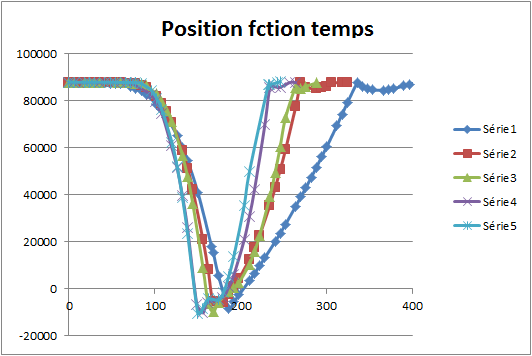
\includegraphics[width=8.3cm]{m1_pos.png}
         \caption{Graphique de position en fonction du temps}
     \end{minipage}
     \hfill%
     \begin{minipage}[c]{.46\linewidth}
         \centering
         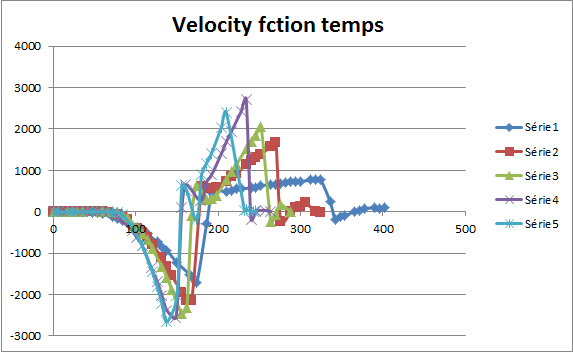
\includegraphics[width=9cm]{m1_speed.png}
         \caption{Graphique de vitesse en fonction du temps}
     \end{minipage}
     \hfill%
     \begin{minipage}[c]{.46\linewidth}
         \centering
         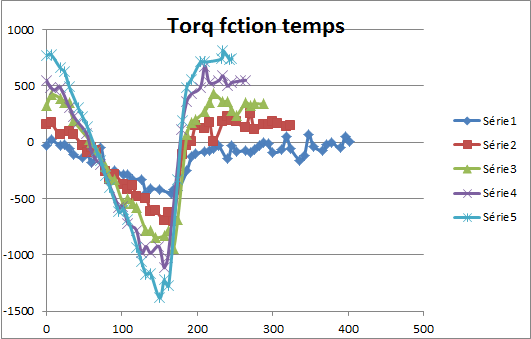
\includegraphics[width=8.3cm]{m1_torque.png}
         \caption{Graphique d'accélération en fonction du temps}
     \end{minipage}
     \hfill%
     \begin{minipage}[c]{.46\linewidth}
         \centering
         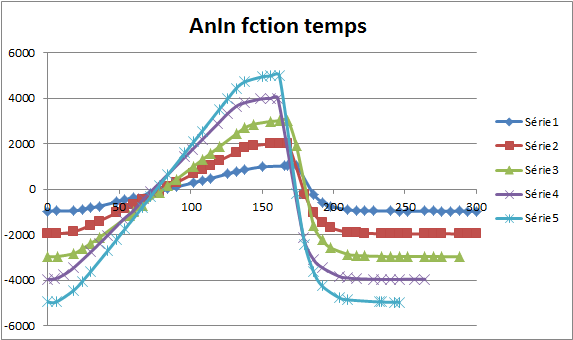
\includegraphics[width=9cm]{m1_AnIn.png}
         \caption{Graphique des entrées analogique en fonction du temps}
     \end{minipage}
 	\end{figure}} 
		
	Dans un premier temps, pour chacun des graphiques ci-dessus, on peut observer une évolution des courbes, qui paraît être en accord avec le comportement attendu. Ainsi, que l'on analyse le mode de position, de vitesse, ou d'accélération, on peut observer que l'ensemble des courbes décroissent de plus en plus rapidement, plus le niveau de tension appliqué devient élevé. Il en va de même pour les courbes du graphique de l'entrée analogique en fonction du temps, plus le niveau de tension augmente, plus la pente des rampes devient importante. Ainsi, jusqu'içi, nous restions plutôt confiants.
	
	Par la suite, nous avons commencé à nous intéresser et nous concentrer sur le mode de contrôle en accélération (mode torque) de notre contrôleur. En effet, étant donné qu'à l'aide de notre module, nous captons le signal d'accélération de la touche de notre piano, l'utilisation du contrôle en accélération (torque) de notre contrôleur nous parut comme étant un choix intéressant et logique pour le contrôle des moteurs; nous permettant de travailler sur les données brutes du signal d'accéléromètre, 	sans besoin de l'intégre pour en obtenir la vitesse, et donc d'intégrer avec ce dernier, des erreurs.
	
	Étant donné que les données sont obtenues par intégrations successives, donc par sommes successives, les mesures ne peuvent pas être prises réellement en continu; donc, les sommes introduiront nécessairement de petites erreurs. D'autre part, même avec une mesure parfaitement exacte de l'accélération, on se retrouve avec une estimation de la vitesse qui dérive petit à petit, en fonction des erreurs accumulées. La position est obtenue en intégrant la vitesse, y compris son erreur d'intégration. Ainsi, l'erreur de position sera quadratique par rapport aux approximations initiales. 
	
	C'est pour cette raison, que nous nous sommes appliqué à mettre en place le contrôle en accélération sur notre contrôleur. Mais avant d'implanter cette solution, nous avons tout de même cherché à vérifier si se dit mode de contrôle en accélération (mode torque), appliquait au moteur un comportement image de l'accélération mesuré. Même si ce mode de contrôle paraissait être "idéal" pour le projet, un premier élément attira notre attention. Ce mode de contrôle en accélération étant nommé contrôle "Torque", il traduirait l'application d'un couple sur notre moteur, pour mettre ce dernier en mouvement, hors un couple appliqué à un moteur en translation, paraît quelque peut contradictoire.
	Une fois la documentation du contrôleur vérifié, il s'avère que ce mode de contrôle "Torque" soit un asservissement numérique sous la forme d'un correcteur Proportionnel Intégral (PI) en courant; ce dernier combinant l'action des correcteurs précédents pour améliorer les performances globales du système asservi. Mais, bien qu'étant un asservissement en courant, une solution de contrôle plutôt aisé à mettre en oeuvre, serait de comparer la courbe du contrôle en accélération avec la courbe de la deuxième dérivée du contrôle en position. En procédant ainsi, nous devrions avoir deux courbes ayant la même allure, permettant ainsi de valider le comportement du contrôle en accélération.
	
		\subsection{Caractérisation du mode de contrôle en accélération ou mode "Torque"}

	Souhaitant obtenir une courbe d'accélération en nous basant sur un mode de contrôle en position, il va donc nous falloir dériver deux fois notre fonction, afin d'obtenir une courbe d'accélération exploitable.
	Notre système à dérivé étant une fonction discrète, nous allons calculer sa dérivée première comme suivant: 
	
	\[	
		f'(x) = \frac{f(x+h) - f(x-h)}{2h}
	\]
	
	puis, sa dérivé seconde:
	
	\[	
		f''(x) = \frac{f(x+h) - 2f(x) + f(x-h)}{h^2}
	\]
	
	
		\textsc{\begin{figure}[h]
    	\begin{minipage}[c]{.46\linewidth}
         \centering
         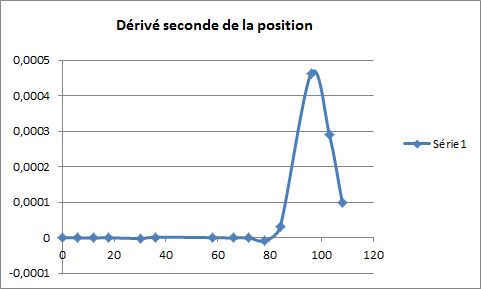
\includegraphics[width=8.3cm]{fscd.png}
         \caption{Graphique de la dérivé seconde de la position en fonction du temps}
    	\end{minipage}
     	\hfill%
     	\begin{minipage}[c]{.46\linewidth}
         \centering
         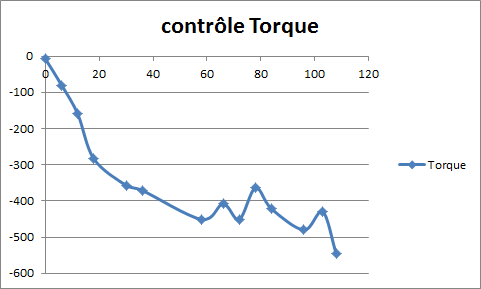
\includegraphics[width=9cm]{torque.png}
         \caption{Graphique de l'accélération en fonction du temps}
    	\end{minipage}
		\end{figure}}
		
		Grâce aux graphiques ci-dessous, nous pouvons nous apercevoir que nos deux graphiques ont une allure en rien comparable, jetant un doute sur le fonctionnement du mode "torque" de notre contrôleur moteur; posant la question du rôle de ce mode de contrôle, si ce dernier n'est pas destiné à être image d'un contrôle en accélération.
		De plus, outre la non-adéquation avec le mode de contrôle "Torque", nous nous sommes demandé si le traitement du signal analogique par le contrôleur moteur, pouvait ou non, induire un retard, un décalage temporel entre la consigne mesurée et l'établissement de la valeur de contrôle en sortie du contrôleur.
		
		\subsection{Du retard induit}
		
		Suite à la caractérisation du mode "Torque", comme nous l'avons dit précédemment, l'induction d'un retard entre la consigne mesurée et l'établissement de la valeur de contrôle en sortie du contrôleur, si elle existe, peut être un obstacle à l'établissement de notre fonction de transfère.
		
		Pour cela, à l'aide des données relevées plus tôt à partir des capteurs à effet hall, nous avons tracé de nouveaux graphiques afin de pouvoir visualisé le signal de contrôle, ainsi que le signal de consigne appliquée en entrée du contrôleur en fonction du temps.
		
		Nous avons commencé par appliquer un signal carré avec notre générateur de fonction, d'une amplitude variant d'un volt jusqu'à cinq Volts; en comparant les différents jeux de mesures réalisées sur la même base de temps, on arrive à un retard moyen d'une valeur de douze millisecondes.
		
		Ensuite, nous avons effectué le même test en appliquant une une rampe croissante avec notre générateur de fonction, et nous avons pu observer un retard d'en moyenne 10 millisecondes entre la consigne et le signal de sortie.
		
		\subsection{Conclusion}
		Après avoir cherché à caractériser le comportement du contrôle en accélération de notre contrôleur moteur, puis après avoir observé le retard induit dans notre système par ce même contrôleur moteur, nous pouvons conclure que la manipulation mise en place, ne nous permet pas de pouvoir établir la fonction de transfère de notre module.
		
		Pour cela, nous allons mettre en place une seconde manipulation, dans laquelle le retard n'aura pas d'incidence. De plus, cette manipulation aura aussi l'avantage de nous permettre de mieux caractériser la contrôle "Torque" du contrôleur.
		
		\newpage		
		
	\section{Seconde manipulation}
	
		\subsection{Introduction}
	
		Comme nous avons pu le voir précédemment, lors de la première manipulation, le retard induit par le contrôleur moteur, nous à poser soucis dans la première manipulation. Du fait, de ce retard, il nous était impossible de mettre en place un modèle afin de pouvoir déduire notre fonction de transfère.
		
		Pour cela, nous avons mis en place cette deuxième expérience, qui a pour but de nous permettre de sortir un modèle, au sein du quel le retard n'aurait pas d'incidence; mais ne serait qu'un élément de l'équation à faire varier pour établir notre modèle. Pour cette manipulation, nous avons procédé, comme l'illustre le schéma bloc ci-dessous.		
		
	\begin{figure}[!ht]
    \center
    %\hfill\hbox to 0pt{\hss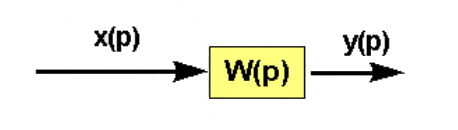
\includegraphics[width=17cm]{transf1.png}\hss}\hfill\null
  	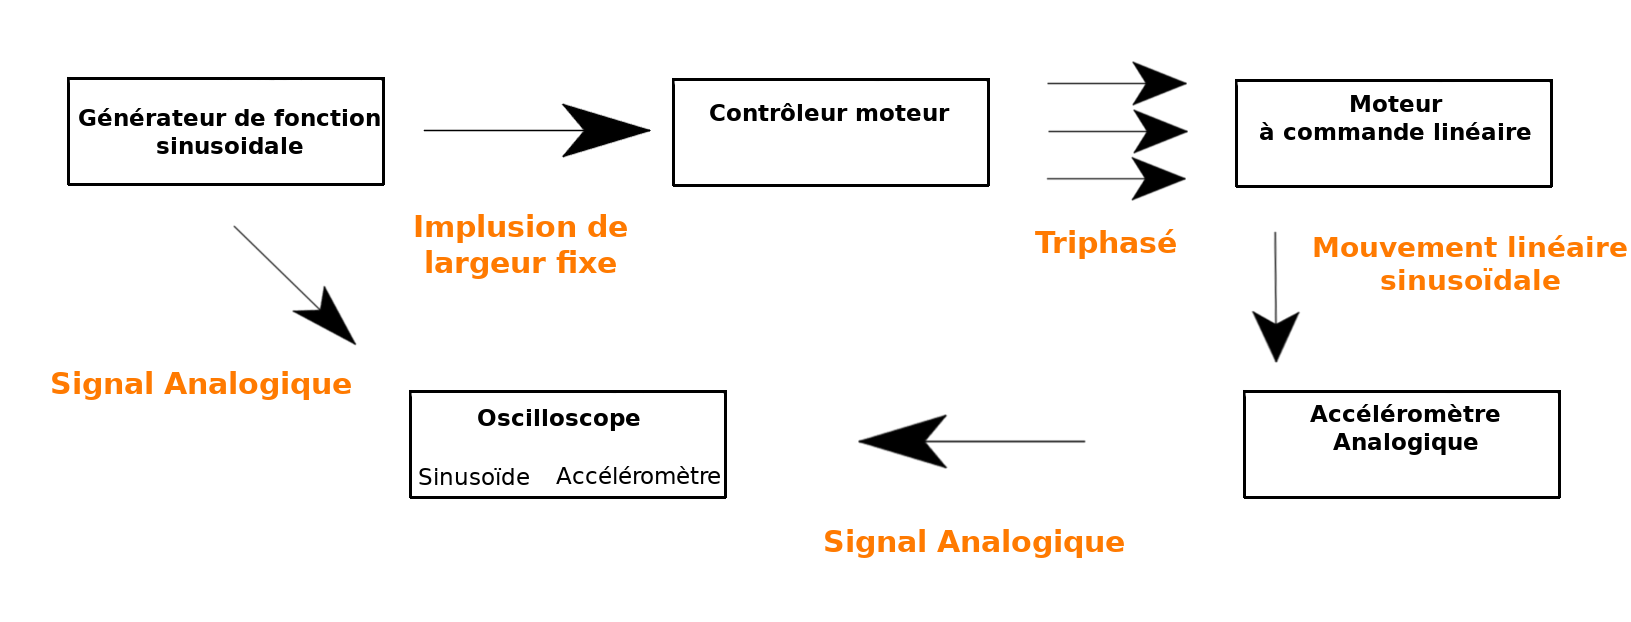
\includegraphics[width=18cm]{manip2.png}
    \caption{Schéma bloc - Seconde manipulation}
	\end{figure}	
	
	Nous utilisons encore une fois notre générateur de fonction afin de générer un signal sinusoïdal à destination de notre contrôleur, ce signal analogique sinusoïdal sera varié selon deux paramètres. Tout d'abord son amplitude, évoluant sur un intervalle de trois Volts jusqu'à cinq Volts, puis c'est la fréquence du signal que nous ferons varier; fréquence qui devra évoluer entre vingt Hertz et 100 Hertz.	Faire varier ces paramètres va nous permettre de vérifier le paramètre ayant une incidence majeure sur le comportement du contrôleur.
	
	De plus, nous avons placé un accéléromètre sur notre bras aimenté, afin de pouvoir tracer sa courbe de réponse sur l'axe "Z" sur notre oscilloscope. Tracer cette courbe de réponse en même temps que la courbe fournie par le générateur de fonction va nous permettre d'observer l'ensemble des différences entre ces deux courbes et d'en déduire le déphasage ainsi que le retard.
	
	Enfin, nous pourrons également mieux tenter de caractériser notre contrôle en accélération, étant donné que nous pourrons comparer des grandeurs physiques de même nature en entrée, comme en sortie du système. Ces données pourront être analysées au travers d'un diagramme de BODE.
	
		\subsection{Traitement des données}
		
		Afin de caractériser notre fonction de transfère, nous avons tout d'abord commencé par représenter sous forme de graphique notre nouveau système, afin de pouvoir observer les différences entre les deux courbes obtenues.
		On retrouve ci-dessous, trois graphiques à titre d'exemple des mesures effectuées; mesures ayant également été prises pour les valeurs de fréquences suivantes : 20Hz, 30Hz, 40Hz, 50Hz, 70Hz et 100Hz. 
		
	\textsc{\begin{figure}[h]
     \begin{minipage}[c]{.46\linewidth}
         \centering
         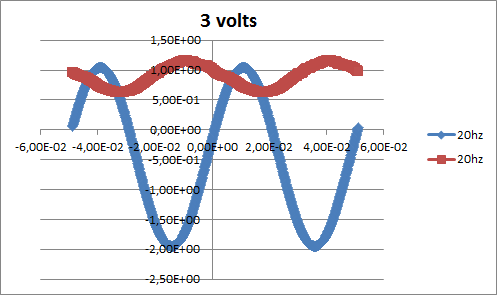
\includegraphics[width=8.3cm]{osciAcc_3v.png}
         \caption{Graphique oscillo - accéléromètre - 20Hz, 3 Volts}
     \end{minipage}
     \hfill%
     \begin{minipage}[c]{.46\linewidth}
         \centering
         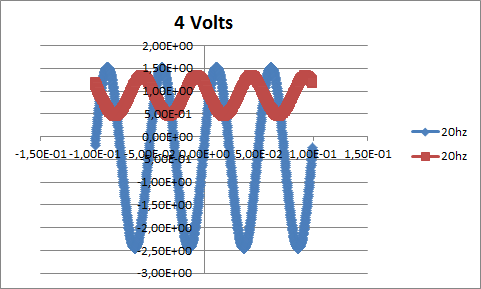
\includegraphics[width=9cm]{osciAcc_4v.png}
         \caption{Graphique oscillo - accéléromètre - 20Hz, 4 Volts}
     \end{minipage}
     \hfill%
     \begin{minipage}[c]{.46\linewidth}
         \centering
        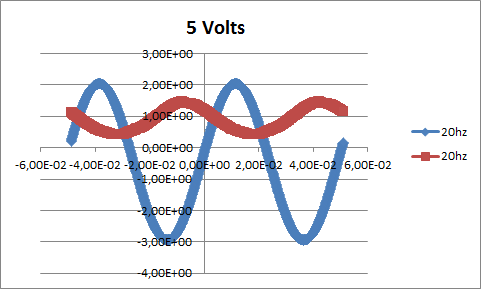
\includegraphics[width=8.3cm]{osciAcc_5v.png}
         \caption{Graphique oscillo - accéléromètre - 20Hz, 5 Volts}
     \end{minipage}
 	\end{figure}}
 	
 	Grâce à nos graphiques ci-dessus, on peut observer que nos deux courbes, image du signal sinusoïdale fournie par le générateur de fonction, ainsi que le signal issu de notre accéléromètre analogique, sont quasiment en opposition de phase (pour un déphasage avoisinant les 180 degrés). Mais pour le moment, il nous est impossible de déterminer si nos courbes sont déphasées ou si le signal analogique de l'accéléromètre est en retard par rapport au signal du générateur de fonction; retard pouvant être dû à notre contrôleur moteur.
 	
 	Afin de déterminer si nous sommes en présence d'un retard, d'un déphasage, ou des deux, nous avons procédé comme suivant.
 	Dans un premier temps, nous avons reconstruit deux signaux sinusoïdaux, en nous basant sur leur équation, afin de pouvoir faire varier leurs paramètres et ainsi en déduire le déphasage et/ou le retard.
 	Le premier signal reconstitué se base sur le signal du générateur de fonction. Dans ce cas-ci, il nous est possible de négliger le retard, étant le signal premier.
	
	\[	
		f(x) = Offset + Ampl * Sin( 2*Pi*F*(T) + Dephasage )
	\]	
	
	Le deuxième est l'image du signal fournie par l'accéléromètre, fonction dans laquelle, nous intégrons cette fois, la notion de retard.
	
	\[	
		f(x) = Offset + Ampl * Sin( 2*Pi*F*(T-retard) + Dephasage )
	\]	
	
	Enfin, nous avons effectué une minimisation sous contrainte sur la fonction sinus, précédemment reconstruite, afin de déterminer les coefficients de déphasage, de retard et d'amplitude, tout en fixant des paramètres tels que l'amplitude et la fréquence. Cette méthode nous a donc permis de déterminer de manière précise, le déphasage entre nos deux courbes, ainsi que les rapports d'amplitudes entre ces dernières, comme nous pouvons l'observer sur la figure ci-dessous:
	
	\begin{figure}[!ht]
    \center
    %\hfill\hbox to 0pt{\hss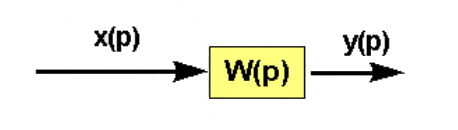
\includegraphics[width=17cm]{transf1.png}\hss}\hfill\null
  	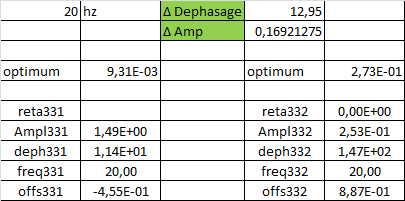
\includegraphics[width=10cm]{dephAmp.png}
    \caption{Minimisation de la fonction sinus}
	\end{figure}	
	
	Disposant maintenant de l'ensemble des rapports d'amplitudes et de déphasages entre nos signaux analogiques, il nous est possible de tracer la courbe de déphasage en fonction de la fréquence et d'Amplitude en fonction de la fréquence.
	 	
		\begin{figure}[!ht]
    \center
    %\hfill\hbox to 0pt{\hss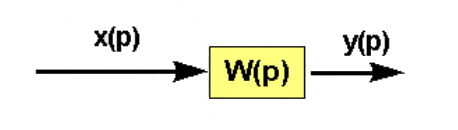
\includegraphics[width=17cm]{transf1.png}\hss}\hfill\null
  	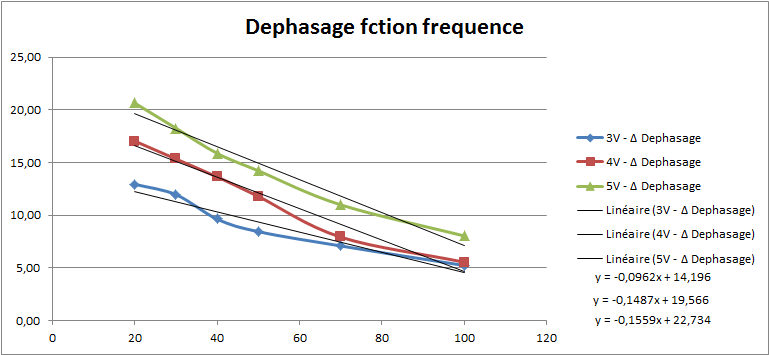
\includegraphics[width=15cm]{dFctionFreq.png}
    \caption{Déphasage en fonction de la fréquence}
	\end{figure}	
	
	\begin{figure}[!ht]
    \center
    %\hfill\hbox to 0pt{\hss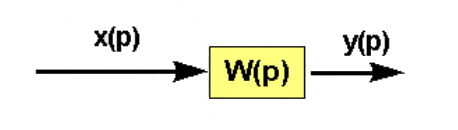
\includegraphics[width=17cm]{transf1.png}\hss}\hfill\null
  	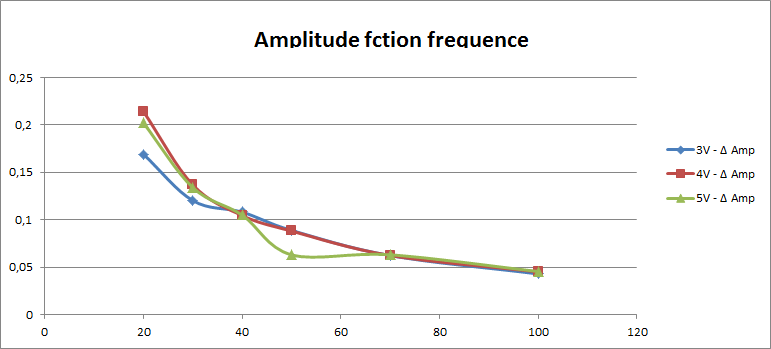
\includegraphics[width=15cm]{AFctionFreq.png}
    \caption{Amplitude en fonction de la fréquence}
	\end{figure}
	
	Grâce aux courbes ci-dessous, on peut observer que nous disposant enfin d'un modèle à partir du quel nous pouvons déterminer une fonction de transfère de notre système. Mais avant cela, il nous reste un dernier graphique à analyser; disposant des rapports d'amplitudes entre nos signaux analogiques, nous pouvons réaliser un diagramme de BODE. Ce diagramme devrait nous permettre de pouvoir caractériser de manière précise notre contrôleur moteur.
	
	\begin{figure}[!ht]
    \center
    %\hfill\hbox to 0pt{\hss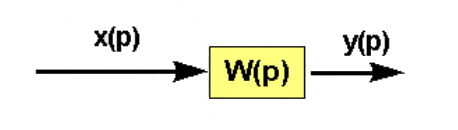
\includegraphics[width=17cm]{transf1.png}\hss}\hfill\null
  	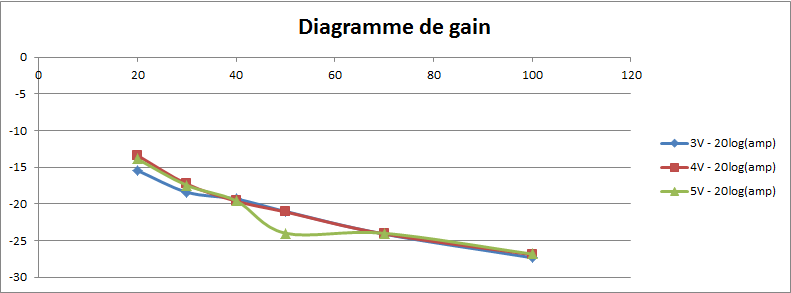
\includegraphics[width=15cm]{baud.png}
    \caption{Diagramme de BODE}
	\end{figure}	
	
	Comme nous pouvons le voir ci-dessus, notre diagramme de BODE qui devrait être horizontale, s'avère avoir une pente de six db/octave, ce qui traduit que nous sommes déjà dans la pente de la bande rejeté, alors que nous sommes très loin de la valeur de la fréquence de coupure étant de 1 KHz.
	
	\begin{figure}[!ht]
    \center
    %\hfill\hbox to 0pt{\hss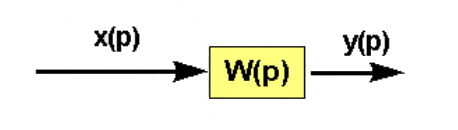
\includegraphics[width=17cm]{transf1.png}\hss}\hfill\null
  	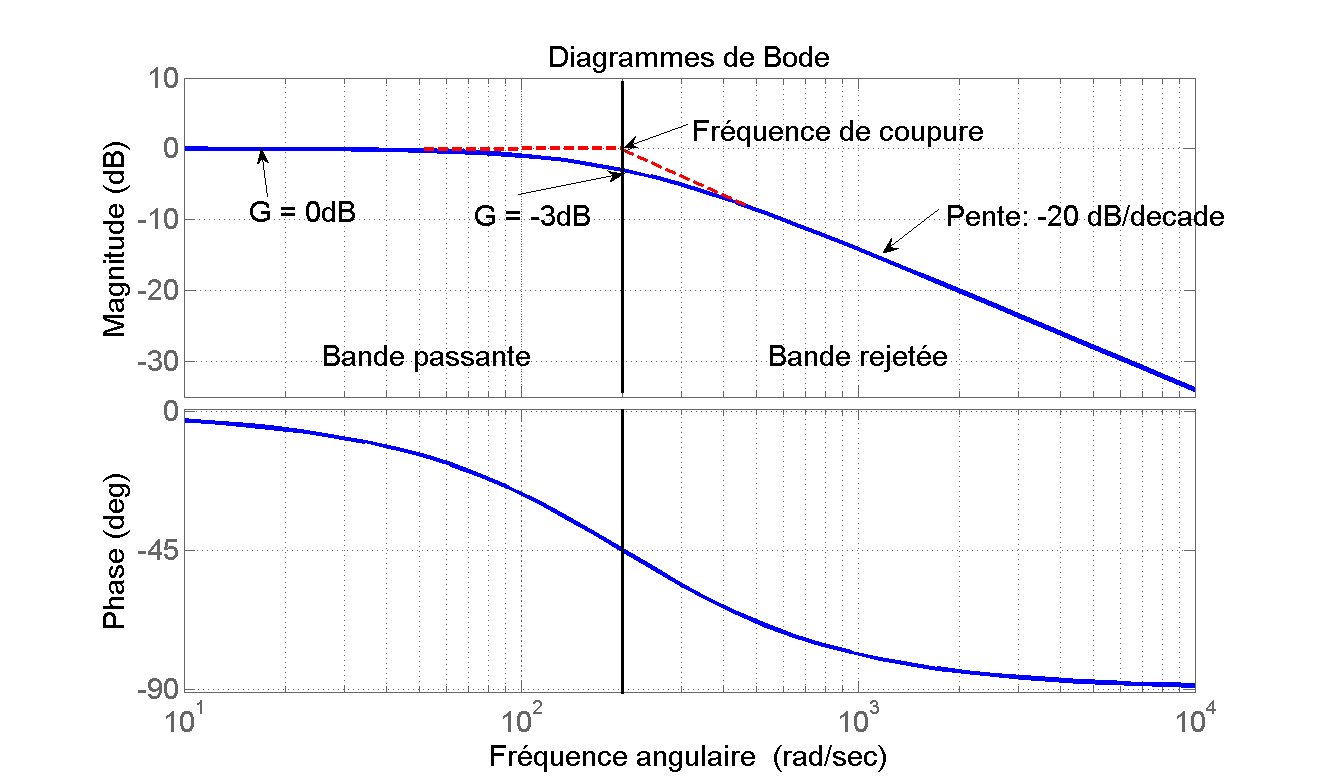
\includegraphics[width=15cm]{bode.png}
    \caption{Diagramme générique de BODE}
	\end{figure}
	
\newpage	
	
		\subsection{Conclusion}
			Après avoir reconstruit des signaux sinusoïdaux, puis avoir effectué une minimisation sous contrainte, afin de pouvoir déterminer les coefficients de déphasage ainsi que les rapports d'amplitudes entre le signal de notre oscilloscope et de notre accéléromètre, nous avons pu réaliser des graphiques nous permettant de déduire une fonction de transfère de notre système.
			
			Mais suite à la modélisation du diagramme de bode, nous pouvons conclure qu'étant déja dans la courbe de fréquence rejetée, le contrôle en accélération de notre contrôleur ne paraît pas être viable, invalidant de ce fait, nos courbes devant nous permettre de déterminer notre fonction de transfère.
			
\newpage
			
		\section{Ouverture}
	
		Etant donnée les échecs connus avec les deux précédentes manipulations, une troisième doit être mise en place afin de déterminer efficacement le contrôle en vitesse du contrôleur.
		
		Pour cela, nous allons procéder comme illustré sur le schéma bloc ci-dessous. La manipulation reprend le même principe que la deuxième, à la différence que nous allons intégrer le signal de l'accéléromètre au sein du FPGA pour fournir au contrôleur une courbe en adéquation avec un contrôle en vitesse.
		
	\begin{figure}[!ht]
    \center
    %\hfill\hbox to 0pt{\hss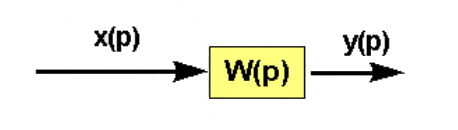
\includegraphics[width=17cm]{transf1.png}\hss}\hfill\null
  	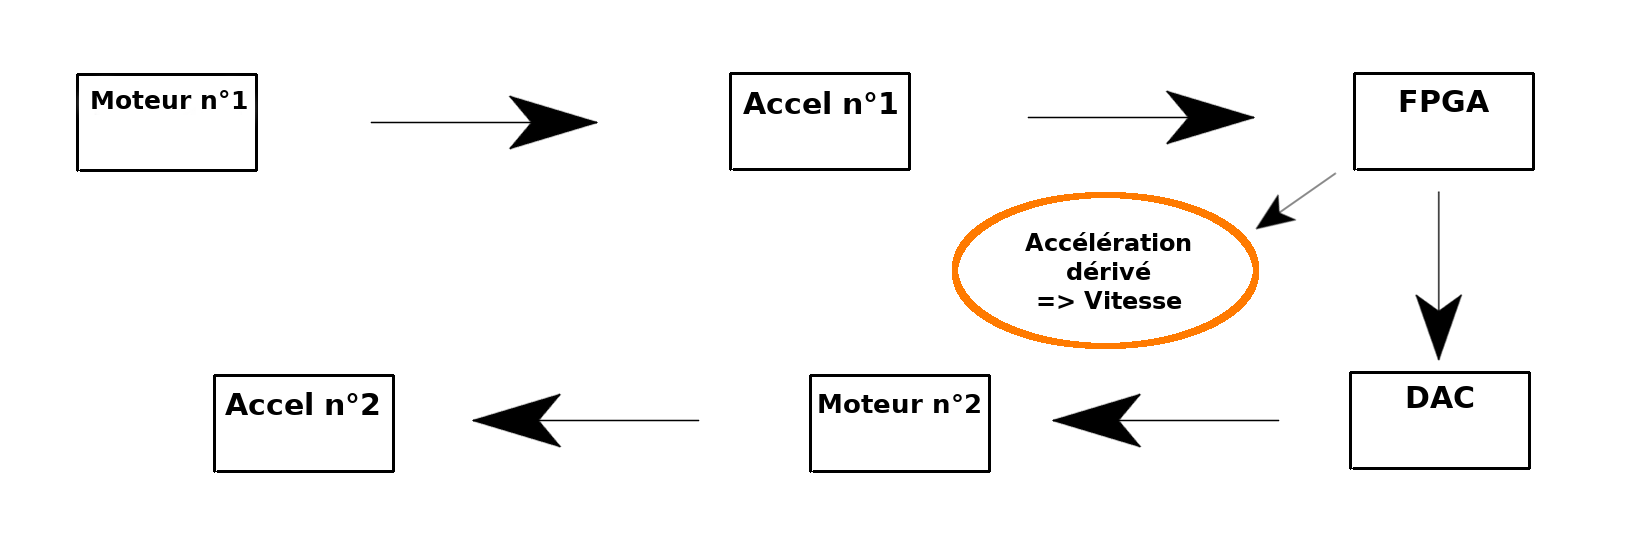
\includegraphics[width=18cm]{manip3.png}
    \caption{Schéma bloc - ouverture manipulation futur}
	\end{figure}
	
	De  plus, le deuxième accéléromètre ne sera pas fixé physiquement sur le deuxième moteur, ce qui va nous permettre de le brancher à divers endroits dans le système afin de pouvoir identifier des sources de déphasage ou de retard. Ainsi, nous pourrons disposer d'une caractérisation très précise de notre système et pouvoir disposer d'une fonction de transfère viable.
	
	
	


	
	
	
	
	
	
	
	
	
%--------------------------------------------------------------------------------------
%
%	Elément de fin de document
%		Bibliographie
%		Table des figures
%
%--------------------------------------------------------------------------------------

\part{Bibliographie}

	\begin{itemize}
		\item Descriptif global du projet: BHLS-CNRS-UPMC-LPNHE-IRCAM.pdf
	\end{itemize}


\part{Table des figures}

	\listoffigures



\end{document}